\documentclass[twoside,final]{hcmut-report}

\usepackage{array,longtable,multirow,tabularx}
\usepackage{enumitem}
\usepackage{float}
\usepackage{tikz}
\usepackage{xcolor}
\usepackage{booktabs}
\coursename{Deep Learning and Its Applications (CO3133)}
\reporttype{Final Report}
\title{Assignment 1 -- Classification on Image, Text, and Multimodal Data}
\advisor{Le Thanh Sach}
\stuname{
  Chu Nguyen Tuan Anh & Student ID 2352022 \emph{(Group HAT)} \\
  Nguyen Quoc Hieu & Student ID 2352344 \emph{(Group HAT)} \\
  Vu Hai Tuan & Student ID 2353280 \emph{(Group HAT)} \\
}
\reportplace{Ho Chi Minh City}
\reporttime{April 2026}

\graphicspath{{graphics/}{assets/image/}{assets/text/}{assets/multimodal/}}

\hfuzz=20pt

\begin{document}
\coverpage

\tableofcontents
\listoffigures
\listoftables
\newpage

\section{Introduction}

This report presents the final results of Assignment 1 for the course \textit{Deep Learning and Its Applications}. The assignment requires classification experiments on three data modalities: \textbf{image}, \textbf{text}, and \textbf{multimodal image-text pairs}. The main goal is to compare representative model families under a fair and reproducible protocol:
\begin{itemize}[leftmargin=*, nosep]
    \item Image: \textbf{CNN} vs \textbf{Vision Transformer (ViT)}
    \item Text: \textbf{RNN} vs \textbf{Transformer}
    \item Multimodal: \textbf{Zero-shot} vs \textbf{Few-shot}
\end{itemize}

Our group (HAT) organizes the report in a standard research format: problem definition, dataset and EDA, methodology, experimental setup, quantitative results, discussion, and conclusion.

\section{Research Objectives and Assignment Alignment}

\subsection{Objectives}
\begin{itemize}[leftmargin=*, nosep]
    \item Build complete pipelines (dataset, dataloader, preprocessing, augmentation, training, evaluation) for all three modalities.
    \item Compare model families using consistent metrics across settings.
    \item Provide analysis beyond raw accuracy, including calibration and error analysis where appropriate.
    \item Deliver reproducible artifacts through GitHub Pages, code repositories, and presentation materials.
\end{itemize}

\subsection{Alignment with Assignment Brief}
The final report satisfies the technical requirements specified in the assignment brief:
\begin{itemize}[leftmargin=*, nosep]
    \item \textbf{Image track:} comparison between CNN and ViT pretrained models.
    \item \textbf{Text track:} comparison between RNN-based and Transformer-based models.
    \item \textbf{Multimodal track:} comparison between zero-shot and few-shot approaches.
    \item \textbf{Metrics:} accuracy and F1 are consistently reported; precision and confusion matrices are included where useful.
\end{itemize}

\section{Datasets and Exploratory Data Analysis (EDA)}

\subsection{Image Dataset: Stanford Dogs}
\noindent \textbf{Problem context} Stanford Dogs is used for image classification in the image track. The task is fine-grained dog-breed recognition, where visual differences between classes are often subtle and highly localized. This makes the benchmark suitable for comparing a CNN family (ResNet-50) and a Transformer family (ViT-B/16) under the same transfer-learning protocol.\\

\noindent \textbf{Dataset information} Stanford Dogs contains 20,580 RGB images from 120 breeds. The notebook reconstructs the official split from \texttt{train\_list.mat} and \texttt{test\_list.mat}, then creates an internal validation split from the official training partition. In addition, the EDA exports \texttt{metadata\_with\_quality.csv} and \texttt{split\_metadata.csv} so that geometry, color statistics, and split assignments can be inspected separately from the training loop.\\

\noindent \textbf{Official split files and folder structure} The files \texttt{train\_list.mat} and \texttt{test\_list.mat} are MATLAB annotation files distributed with Stanford Dogs. They do not store image pixels; instead, they store relative image paths and class labels that define the official train/test split. The notebook reads these files first, then resolves image paths under the extracted dataset directory. A simplified dataset layout is shown below.

\begin{center}
\fbox{%
\begin{minipage}{0.72\textwidth}
\vspace{0.4em}
\ttfamily
stanford\_dogs/\\
\hspace*{1.5em}Images/\\
\hspace*{1.5em}Annotation/\\
\hspace*{1.5em}lists/train\_list.mat\\
\hspace*{1.5em}lists/test\_list.mat
\vspace{0.4em}
\end{minipage}%
}
\end{center}

\begin{table}[H]
\centering
\caption{Stanford Dogs Dataset Statistics}
\begin{tabular}{lr}
\toprule
\textbf{Statistic} & \textbf{Value / Info} \\
\midrule
Total images & 20,580 \\
Number of classes & 120 breeds \\
Official train split & 12,000 \\
Official test split & 8,580 \\
Min images / class & 148 \\
Max images / class & 252 \\
Mean images / class & 171.5 \\
Mean image width & 442.5 px \\
Mean image height & 385.9 px \\
Mean aspect ratio & 1.187 \\
\bottomrule
\end{tabular}
\label{tab:stanford_dogs_stats}
\end{table}

\begin{table}[H]
\centering
\caption{Main EDA CSV Artifacts Used in the Image Track}
\small
\begin{tabularx}{0.96\textwidth}{>{\raggedright\arraybackslash}p{4.2cm} >{\raggedright\arraybackslash}X}
\toprule
\textbf{Artifact} & \textbf{Main role in the notebook and report} \\
\midrule
\begin{tabular}[t]{@{}l@{}}\texttt{metadata\_with\_quality}\\\texttt{.csv}\end{tabular} & Master per-image metadata table. It keeps the official split identity, relative image path, breed label, geometry statistics, and image-quality descriptors such as brightness, contrast, saturation, and RGB means. This file supports the dataset-level EDA plots and summary statistics. \\
\texttt{split\_metadata.csv} & Final train/validation/test table after stratified validation splitting. It is the bridge between the EDA stage and the DataLoader stage because it records which image is assigned to each final split. \\
\bottomrule
\end{tabularx}
\label{tab:stanford_dogs_eda_artifacts}
\end{table}

\begin{table}[H]
\centering
\caption{Image-Quality Summary from \texttt{metadata\_with\_quality.csv}}
\begin{tabular}{lr}
\toprule
\textbf{Metric} & \textbf{Value} \\
\midrule
Mean brightness & 0.4522 \\
Mean contrast std & 0.2261 \\
Mean saturation & 0.3047 \\
Mean $R$ channel & 0.4761 \\
Mean $G$ channel & 0.4518 \\
Mean $B$ channel & 0.3910 \\
\bottomrule
\end{tabular}
\label{tab:stanford_dogs_quality_stats}
\end{table}

\noindent \textbf{Why the EDA matters before preprocessing} The EDA stage is not only descriptive. It tells us whether the benchmark is balanced enough for stratified splitting, how large the geometric variation is before resizing, whether the dataset has channel imbalance that justifies normalization, and whether the images are visually consistent enough for transfer learning from ImageNet-pretrained models. This is why the report separates raw-input analysis from the actual preprocessing recipe.\\

\begin{figure}[H]
\centering
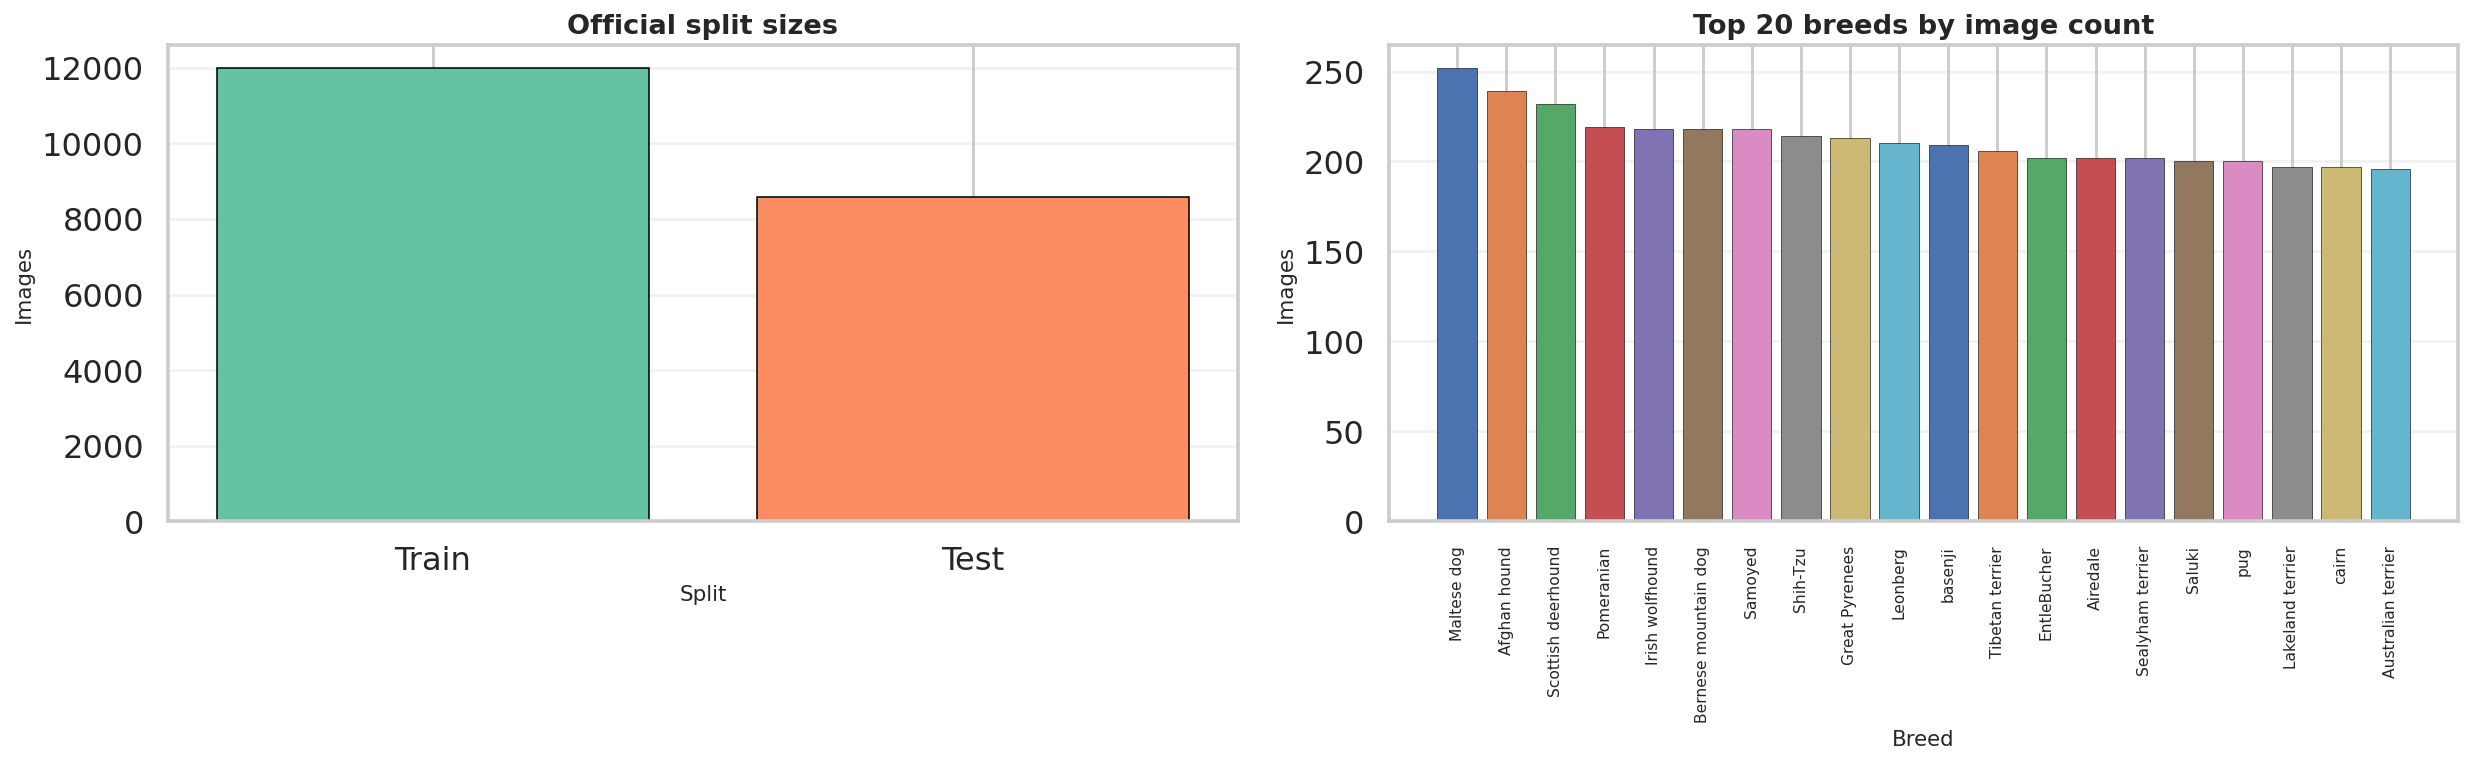
\includegraphics[width=0.78\textwidth]{stanforddogs_dataset_distributions.png}
\caption{Dataset-level distribution summary exported during the Stanford Dogs EDA stage.}
\label{fig:stanforddogs_dataset_distributions}
\end{figure}

\begin{figure}[H]
\centering
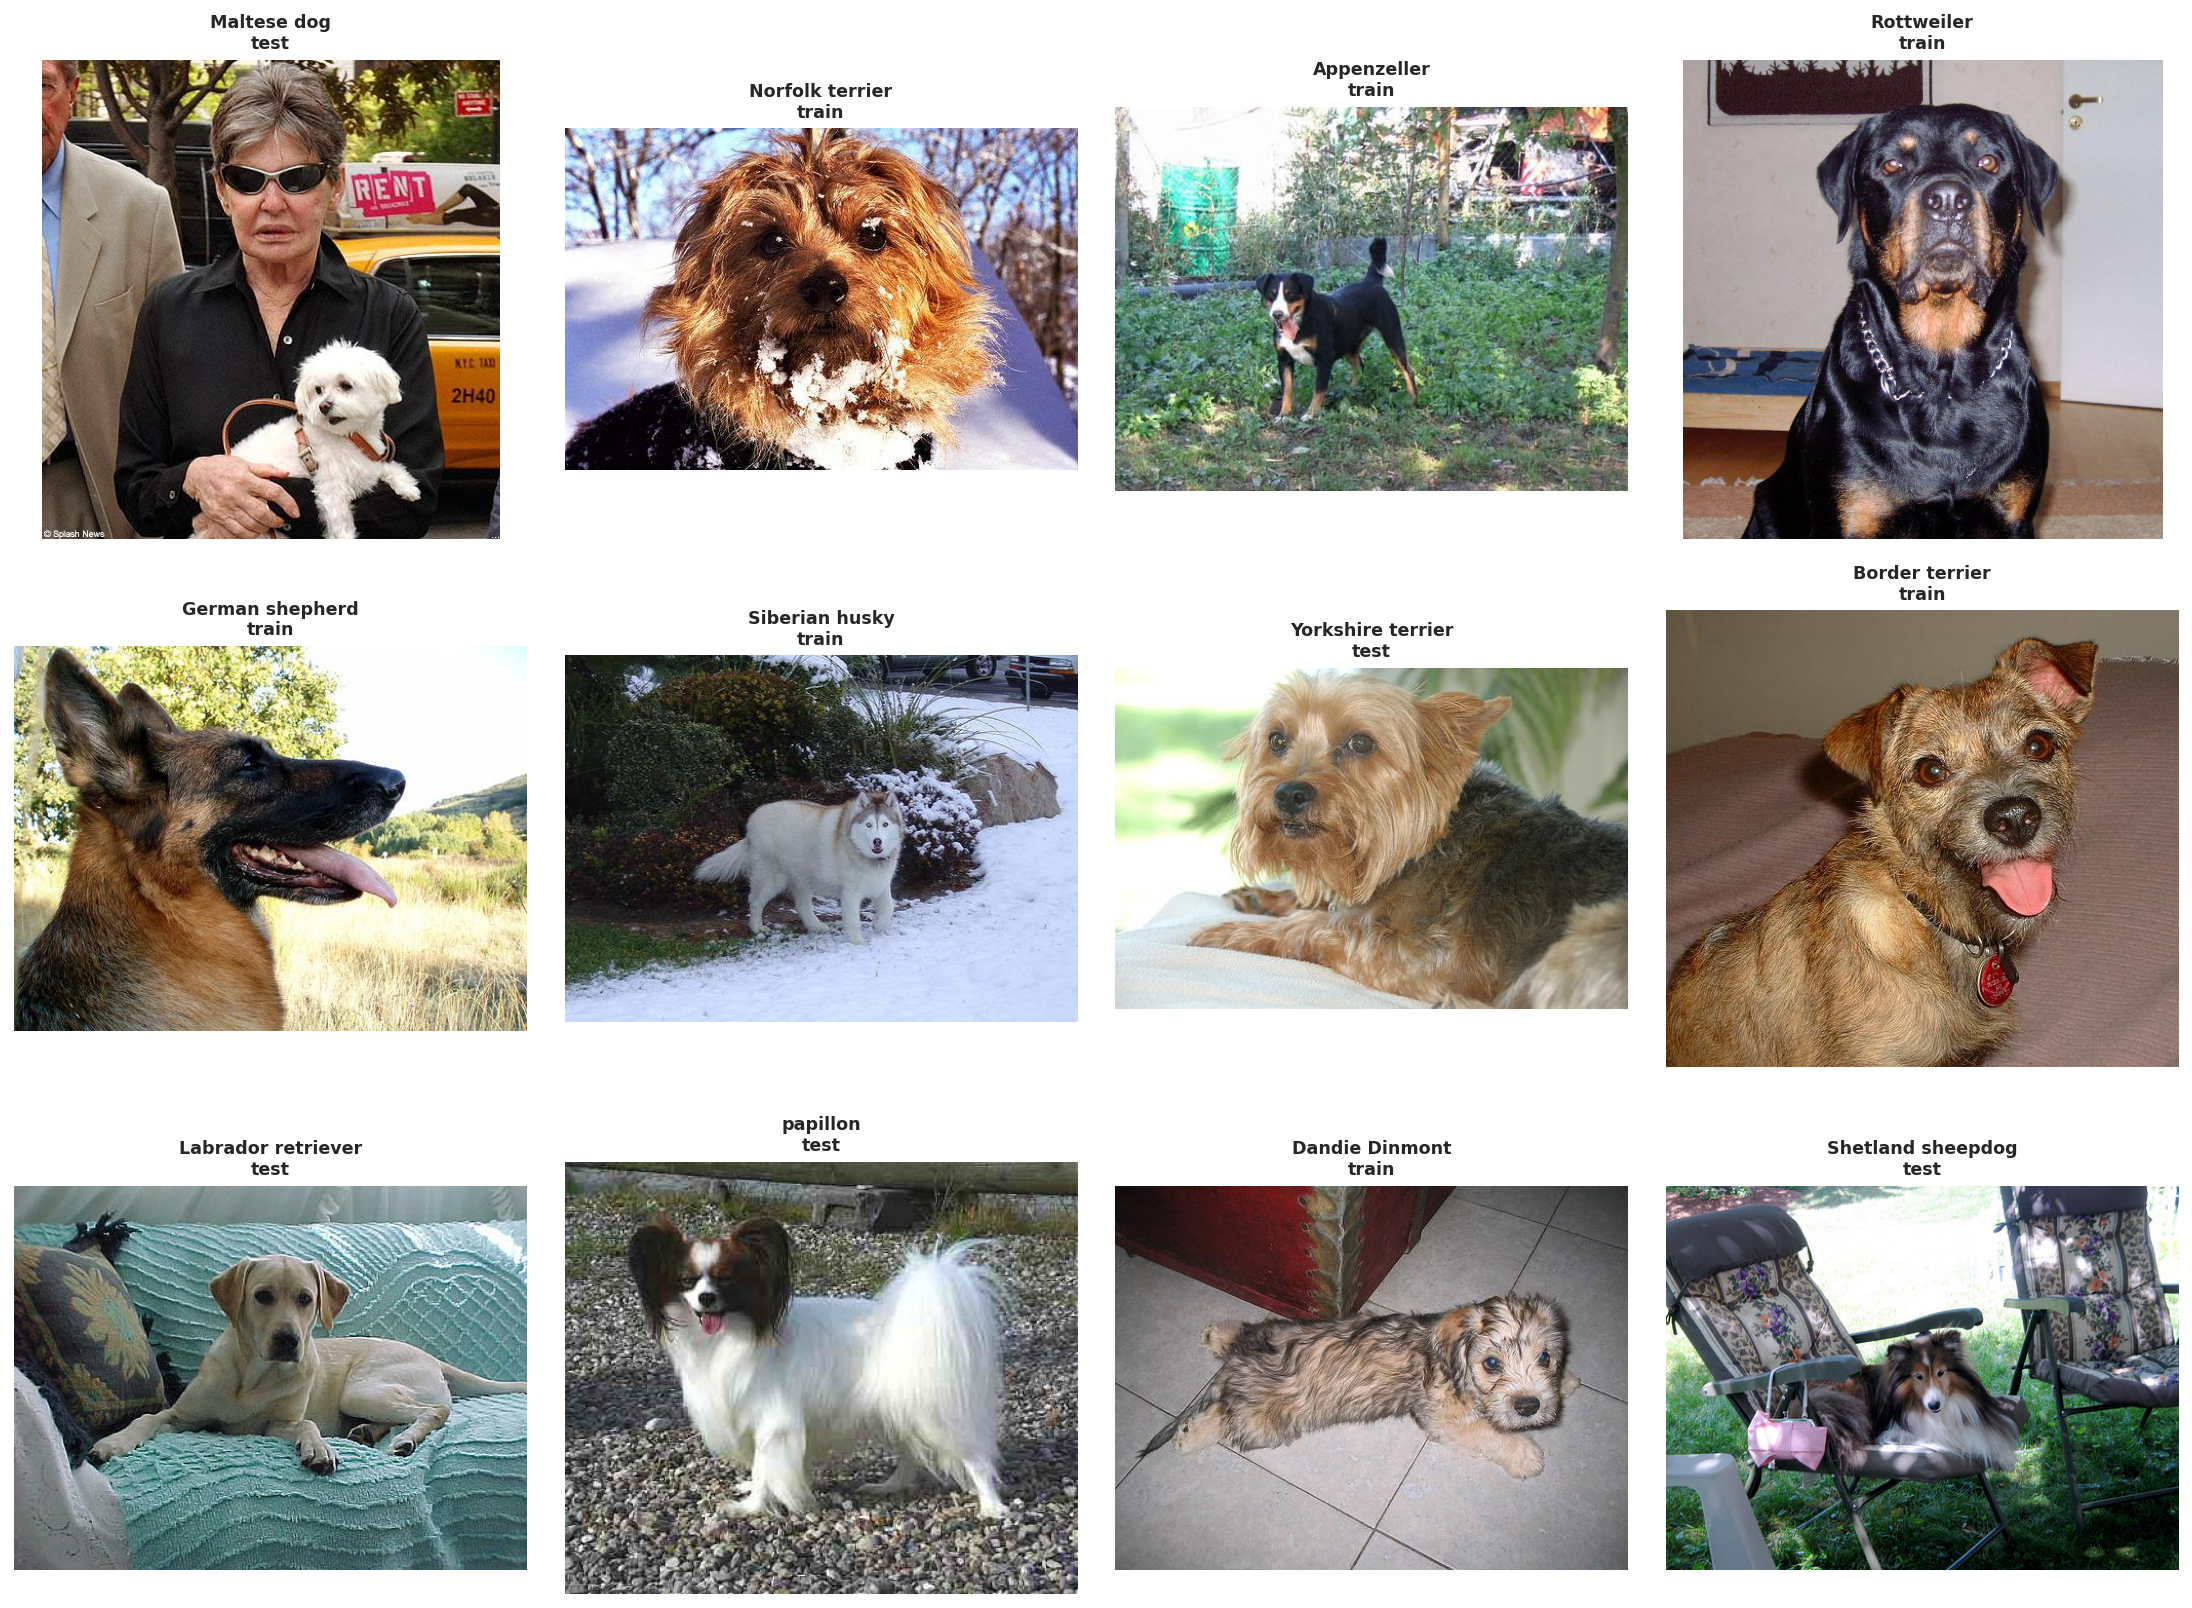
\includegraphics[width=0.92\textwidth]{stanforddogs_random_class_samples.png}
\caption{Random breed samples from Stanford Dogs, illustrating the fine-grained nature of the task.}
\label{fig:stanforddogs_random_class_samples}
\end{figure}

\begin{figure}[H]
\centering
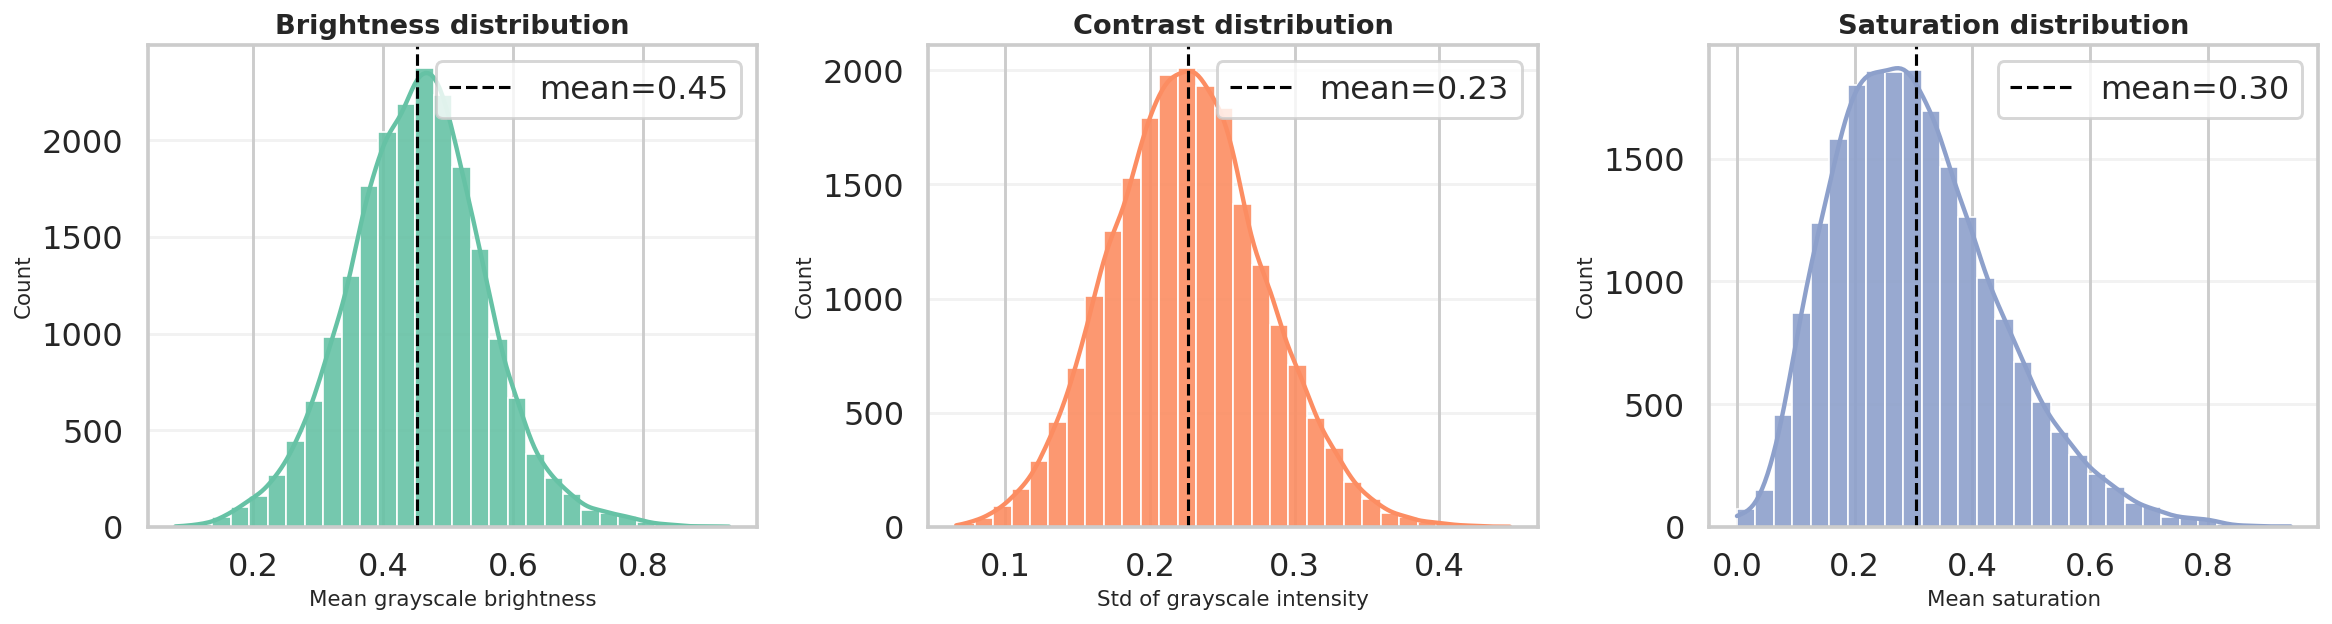
\includegraphics[width=0.82\textwidth]{quality_distributions.png}
\caption{Brightness, contrast, and saturation distributions.}
\label{fig:stanforddogs_quality_distributions}
\end{figure}

\begin{figure}[H]
\centering
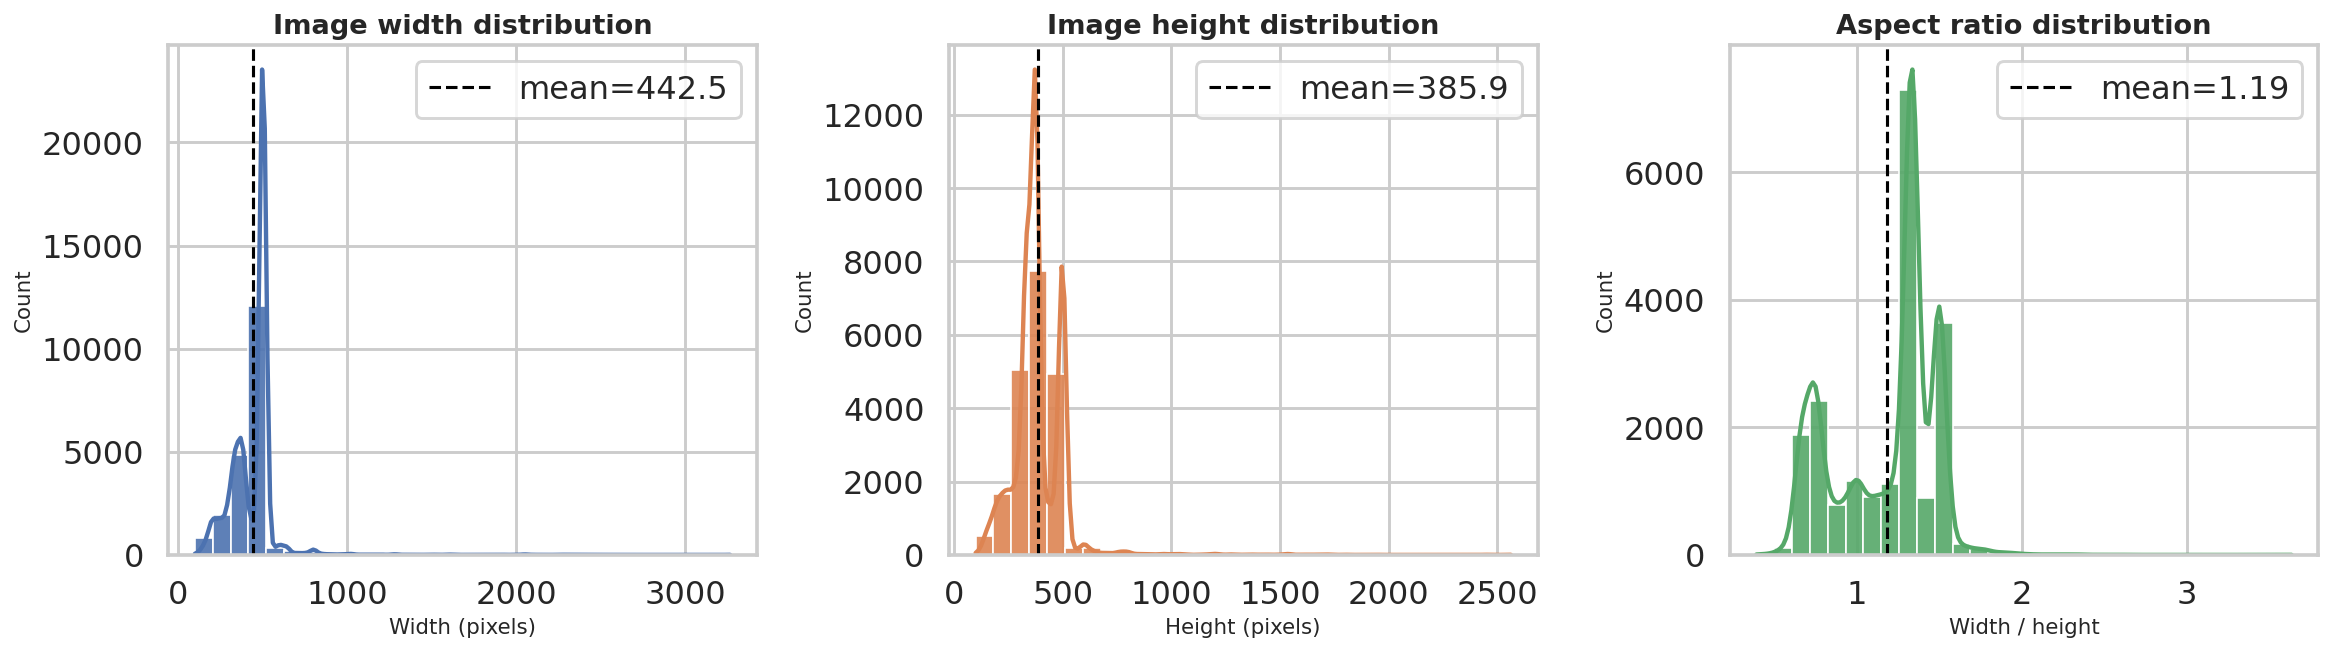
\includegraphics[width=0.82\textwidth]{image_size_distribution.png}
\caption{Image width, height, and aspect-ratio distributions before preprocessing.}
\label{fig:stanforddogs_image_size_distribution}
\end{figure}

\begin{figure}[H]
\centering
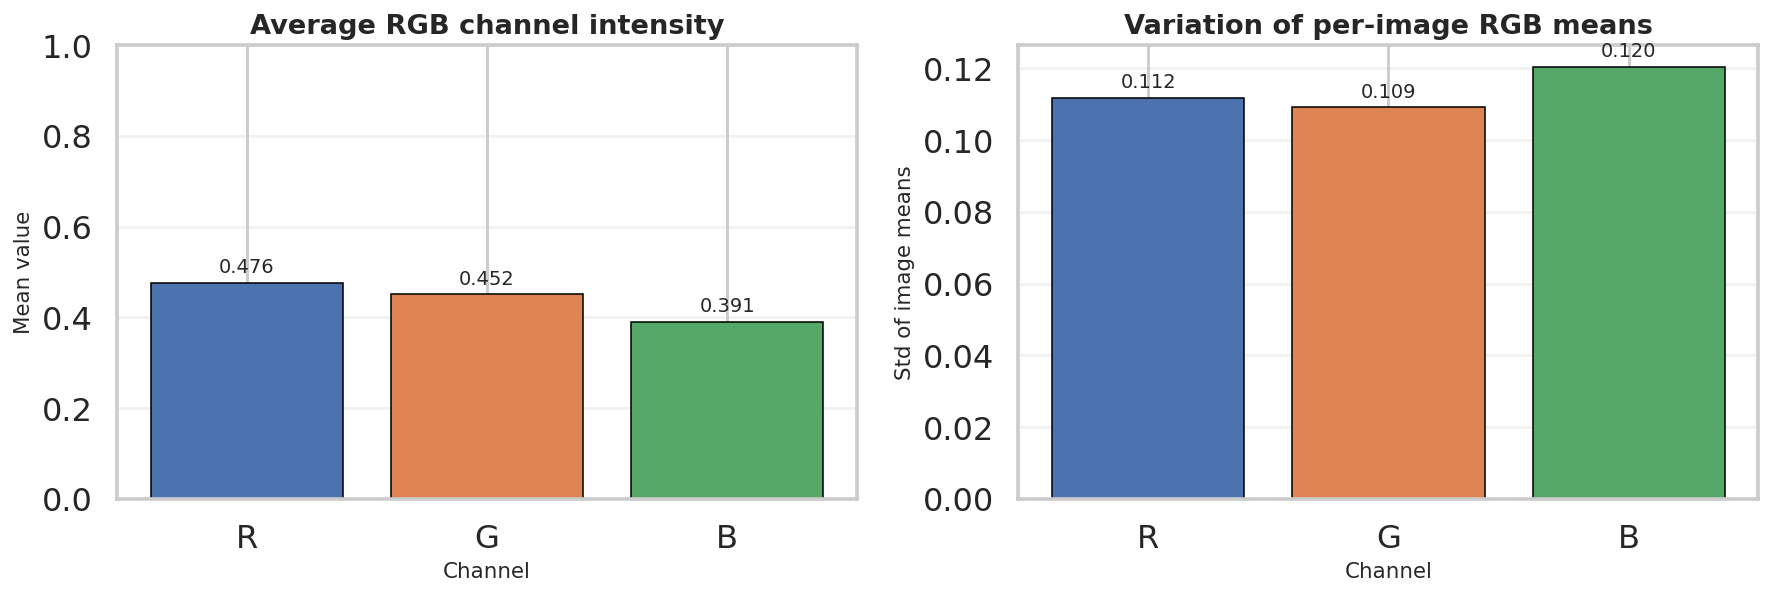
\includegraphics[width=0.82\textwidth]{rgb_channel_summary.png}
\caption{RGB channel summary showing that Stanford Dogs is not perfectly color-balanced before normalization.}
\label{fig:stanforddogs_rgb_channel_summary}
\end{figure}

\subsection{Text Dataset: 20 Newsgroups}
20 Newsgroups is used for topic classification with 20 classes and over 18,000 documents. It provides sufficient class diversity and realistic semantic overlap for comparing BiLSTM and Transformer fine-tuning.

\subsection{Multimodal Dataset: UPMC-Food101 Subset}
For multimodal classification, we use paired image-text samples from a 10-class subset of UPMC-Food101. The dataset contains genuine image-caption/title pairs, which satisfies the multimodal requirement of semantic alignment between modalities.

\section{Methodology}

\subsection{Image Track: ResNet-50 vs ViT-B/16}
We compare two pretrained families under a fair benchmark protocol:
\begin{itemize}[leftmargin=*, nosep]
    \item \textbf{ResNet-50} as the CNN baseline.
    \item \textbf{ViT-B/16} as the Transformer-based vision model.
\end{itemize}
Each family is trained with two strategies:
\begin{itemize}[leftmargin=*, nosep]
    \item \textbf{Full fine-tuning for 12 epochs}
    \item \textbf{Head 3 epochs + full fine-tune 8 epochs}
\end{itemize}
Images are standardized to $224 \times 224$ after resize/crop preprocessing and normalized with ImageNet statistics to match the pretrained checkpoints. The CNN branch uses slightly stronger augmentation, while the ViT branch uses a milder policy to preserve fine-grained breed cues.

Both backbones are initialized from ImageNet-pretrained checkpoints and adapted to 120 Stanford Dogs classes by replacing the final classifier head. For ResNet-50, the final fully connected layer is replaced with a new 120-way linear head. For ViT-B/16, the classification head on top of the CLS-token representation is replaced with a new 120-way output layer. To ensure a fair comparison, the two families share the same split (10,200 train / 1,800 validation / 8,580 test), input resolution ($224 \times 224$), and batch size (32), while both are evaluated under the same two transfer-learning schedules.\\

Training uses \texttt{CrossEntropyLoss}, \texttt{AdamW}, and cosine annealing learning-rate scheduling. For ResNet-50, the learning rate is $1\times10^{-4}$ for full fine-tuning and $1\times10^{-3} \rightarrow 1\times10^{-4}$ for the staged schedule. For ViT-B/16, the learning rate is $3\times10^{-5}$ for full fine-tuning and $1\times10^{-3} \rightarrow 3\times10^{-5}$ for the staged schedule. In all cases, weight decay is set to $1\times10^{-4}$, and the best checkpoint is selected according to validation accuracy. This setup keeps the comparison controlled while still respecting the optimization differences between CNN and Transformer backbones.

\begin{figure}[H]
\centering
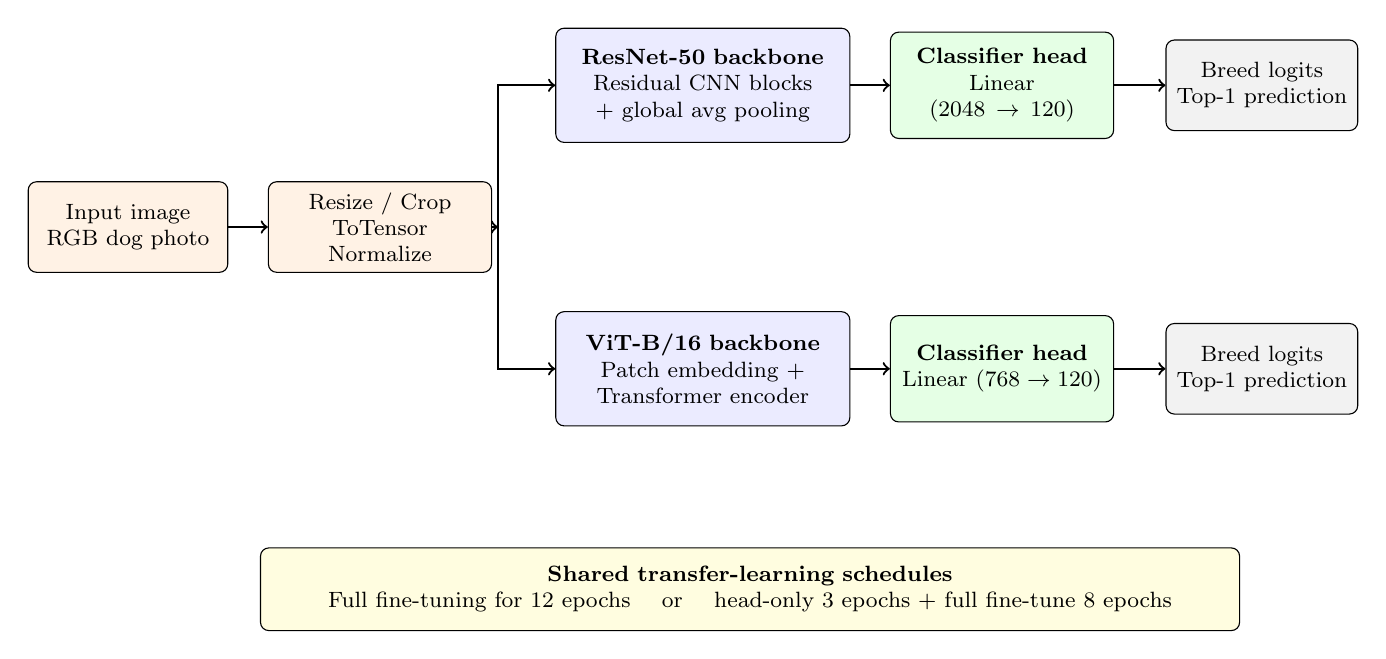
\begin{tikzpicture}[
    font=\footnotesize,
    stage/.style={draw, rounded corners=3pt, align=center, minimum height=1.15cm, text width=2.3cm, fill=orange!10},
    backbone/.style={draw, rounded corners=3pt, align=center, minimum height=1.45cm, text width=3.5cm, fill=blue!8},
    head/.style={draw, rounded corners=3pt, align=center, minimum height=1.35cm, text width=2.6cm, fill=green!10},
    output/.style={draw, rounded corners=3pt, align=center, minimum height=1.15cm, text width=2.2cm, fill=gray!10}
]
\node[stage] (input) at (0,0) {Input image\\RGB dog photo};
\node[stage, text width=2.6cm] (prep) at (3.2,0) {Resize / Crop\\ToTensor\\Normalize};

\node[backbone] (resnet) at (7.3,1.8) {\textbf{ResNet-50 backbone}\\Residual CNN blocks\\+ global avg pooling};
\node[head] (rhead) at (11.1,1.8) {\textbf{Classifier head}\\Linear $(2048 \rightarrow 120)$};
\node[output] (rout) at (14.4,1.8) {Breed logits\\Top-1 prediction};

\node[backbone] (vit) at (7.3,-1.8) {\textbf{ViT-B/16 backbone}\\Patch embedding +\\Transformer encoder};
\node[head] (vhead) at (11.1,-1.8) {\textbf{Classifier head}\\Linear $(768 \rightarrow 120)$};
\node[output] (vout) at (14.4,-1.8) {Breed logits\\Top-1 prediction};

\coordinate (branch) at (4.7,0);

\draw[->, thick] (input) -- (prep);
\draw[->, thick] (prep.east) -- (branch);
\draw[thick] (branch) |- ([xshift=-1.9cm]resnet.center);
\draw[thick] (branch) |- ([xshift=-1.9cm]vit.center);
\draw[->, thick] ([xshift=-1.9cm]resnet.center) -- (resnet.west);
\draw[->, thick] ([xshift=-1.9cm]vit.center) -- (vit.west);
\draw[->, thick] (resnet) -- (rhead);
\draw[->, thick] (rhead) -- (rout);
\draw[->, thick] (vit) -- (vhead);
\draw[->, thick] (vhead) -- (vout);

\node[draw, rounded corners=3pt, align=center, fill=yellow!12, text width=12.2cm, minimum height=1.05cm] at (7.9,-4.6) {\textbf{Shared transfer-learning schedules}\\Full fine-tuning for 12 epochs \quad or \quad head-only 3 epochs + full fine-tune 8 epochs};
\end{tikzpicture}
\caption{Image-track pipeline used in the report. The same preprocessed Stanford Dogs input is sent to either a ResNet-50 CNN backbone or a ViT-B/16 Transformer backbone, then mapped to a 120-class classifier head.}
\label{fig:image_pipeline_backbone_head}
\end{figure}

\subsection{Text Track: BiLSTM + Attention vs DistilBERT}
\begin{itemize}[leftmargin=*, nosep]
    \item \textbf{BiLSTM + Attention}: recurrent baseline with sequence modeling and attention aggregation.
    \item \textbf{DistilBERT}: Transformer backbone fine-tuned end-to-end for classification.
\end{itemize}
The text pipeline includes cleaning, truncation, stratified splitting, dynamic padding, and class-weighted cross-entropy to reduce imbalance effects.

\subsection{Multimodal Track: CLIP Zero-shot vs Few-shot}
CLIP is used as the shared multimodal backbone.
\begin{itemize}[leftmargin=*, nosep]
    \item \textbf{Zero-shot}: prompt-based class matching in the CLIP embedding space.
    \item \textbf{Few-shot}: adaptation with two heads, \textbf{Linear} and \textbf{Prototype}, under 5-shot and 10-shot settings with/without augmentation.
\end{itemize}
The main backbone is CLIP ViT-B/16; CLIP RN50 is reported as an extension.

\section{Experimental Setup}

\subsection{Preprocessing and DataLoader}
Each track uses a dedicated preprocessing pipeline with fixed random seed and stratified splitting where applicable. DataLoaders are configured to ensure fair comparison across models in the same modality.

\subsection{Evaluation Metrics}
Primary metrics are \textbf{Accuracy} and \textbf{F1-score} (macro or weighted depending on context). We also report precision, confusion matrices, and calibration metrics (ECE/reliability diagrams) in extension analysis.

\section{Results and Discussion}

\subsection{Image Track --- Stanford Dogs, ResNet-50, and ViT-B/16}

\subsubsection{Dataset, DataLoader, and Setup}
\noindent \textbf{Split construction} After reading the official split files, the notebook creates a stratified validation set from the official training partition. This gives the final benchmark split shown below.

\begin{table}[H]
\centering
\caption{Train/Validation/Test Split for Stanford Dogs}
\begin{tabular}{lrrl}
\toprule
\textbf{Split} & \textbf{Samples} & \textbf{Loader Batches} & \textbf{Note} \\
\midrule
Train & 10,200 & 319 & Stratified from \texttt{official\_train} \\
Validation & 1,800 & 57 & Stratified from \texttt{official\_train} \\
Test & 8,580 & 269 & Official Stanford Dogs test split \\
\bottomrule
\end{tabular}
\label{tab:stanford_dogs_split}
\end{table}

\noindent \textbf{Preprocessing and augmentation} Both families use the same deterministic evaluation path:
\[
\texttt{Resize((256,256))} \rightarrow \texttt{CenterCrop(224)} \rightarrow \texttt{ToTensor()} \rightarrow \texttt{Normalize(ImageNet)}
\]
The training path is family-specific. ResNet-50 uses a stronger augmentation policy with a wider \texttt{RandomResizedCrop} range, horizontal flip, rotation, color jitter, and random erasing. ViT-B/16 uses a milder crop range and lighter perturbation strength to preserve fine-grained breed cues. In all cases, the input is standardized to a $224 \times 224$ tensor and batched with \texttt{batch\_size = 32}.\\

\noindent \textbf{Normalization} Both models are initialized from ImageNet-pretrained checkpoints, so the notebook normalizes RGB channels with ImageNet statistics:
\[
x_{\mathrm{norm}} = \frac{x - \mu}{\sigma}, \quad
\mu=(0.485, 0.456, 0.406), \quad
\sigma=(0.229, 0.224, 0.225)
\]
Although the exported Stanford Dogs metadata shows slightly different dataset RGB means, the pretrained checkpoint expectation is more important here than matching the raw dataset exactly.\\

\begin{figure}[H]
\centering
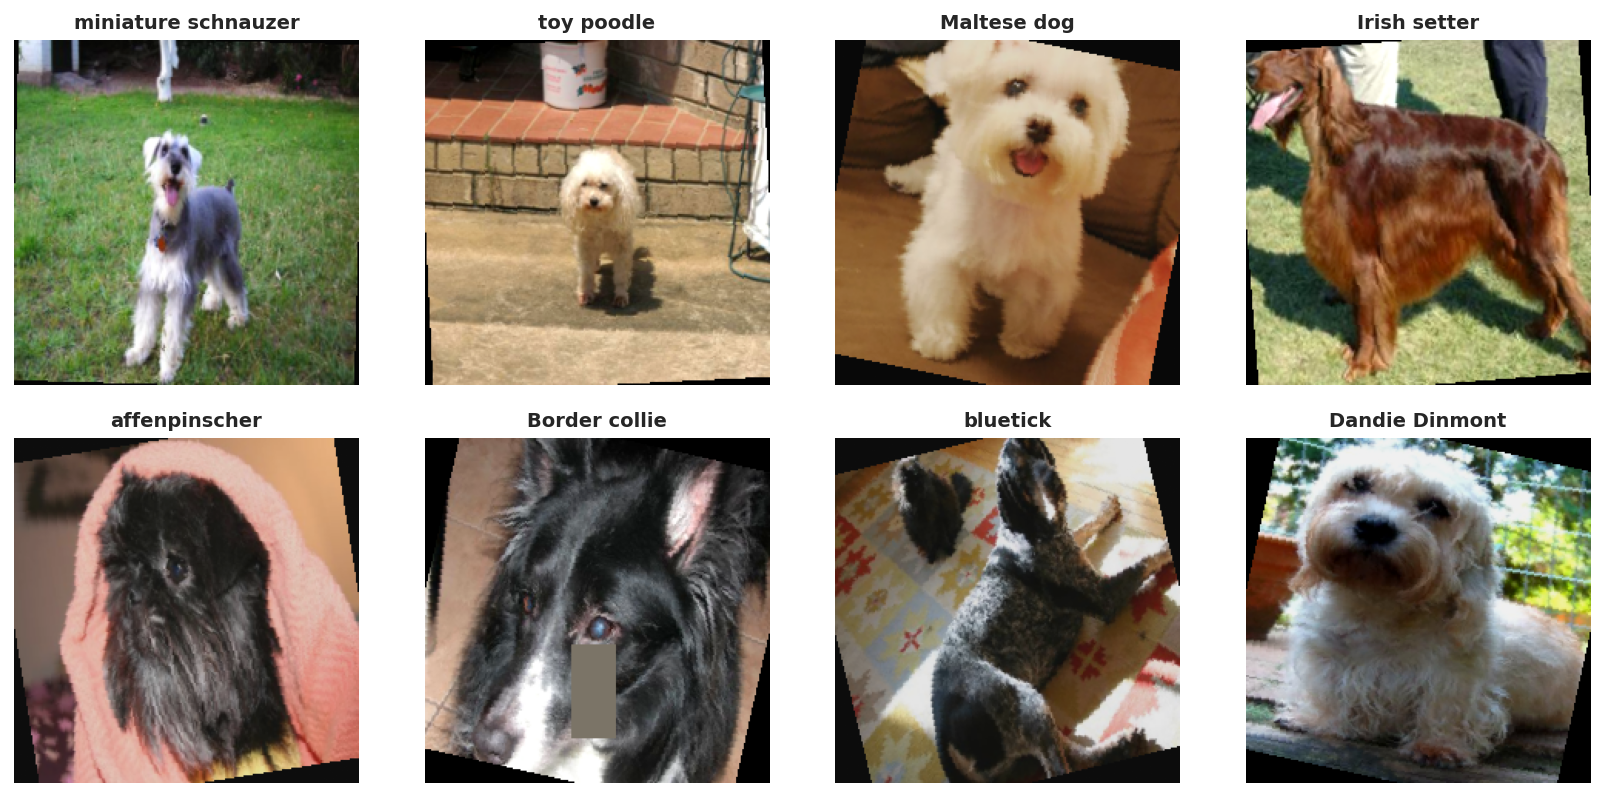
\includegraphics[width=0.84\textwidth]{augmented_batch_preview.png}
\caption{Notebook preview of an augmented training batch after resizing, cropping, tensor conversion, and normalization-aware preprocessing.}
\label{fig:stanforddogs_augmented_batch_preview}
\end{figure}

\subsubsection{Model Building, Training, Evaluation, and Comparison}
\noindent \textbf{ResNet-50} is used as the CNN baseline. The model starts from ImageNet-pretrained weights and replaces the final fully connected layer with a new classifier head for 120 breeds.\\

\noindent \textbf{ViT-B/16} is used as the Transformer baseline. The notebook replaces the head on the CLS token representation and compares the same two transfer-learning schedules used for ResNet-50.\\

\noindent \textbf{Training strategies} To make the comparison fair, each backbone is evaluated with two strategies:
\begin{itemize}[leftmargin=*, nosep]
    \item \textbf{Full fine-tuning for 12 epochs}
    \item \textbf{Head 3 epochs + full fine-tune 8 epochs}
\end{itemize}

\noindent \textbf{Evaluation metrics} The image track reports test accuracy, macro F1, weighted F1, and Expected Calibration Error (ECE). This is important for Stanford Dogs because the benchmark is fine-grained and calibration quality matters in addition to raw classification accuracy.

\begin{table}[H]
\centering
\caption{Image Track Model Summary}
\begin{tabular}{lccc}
\toprule
\textbf{Model} & \textbf{Family} & \textbf{Params} & \textbf{Best Strategy} \\
\midrule
ResNet-50 & CNN & 23.75M & Head 3 + full fine-tune 8 epochs \\
ViT-B/16 & Transformer & 85.89M & Head 3 + full fine-tune 8 epochs \\
\bottomrule
\end{tabular}
\label{tab:image_track_model_summary}
\end{table}

\subsubsection{Experimental Results, Figures, Analysis, and Discussion}
\noindent \textbf{Fair benchmark results} Table~\ref{tab:image_results_stanford_dogs} summarizes the four experiments exported from the final notebook.

\begin{table}[H]
\centering
\small
\begin{tabular}{p{2.3cm} p{4.1cm} c c c c}
\toprule
\textbf{Model} & \textbf{Strategy} & \textbf{Params} & \textbf{Test Accuracy} & \textbf{Macro F1} & \textbf{ECE} \\
\midrule
ResNet-50 & Full fine-tuning (12 epochs) & 23.75M & 85.57\% & 0.8485 & 0.046781 \\
ResNet-50 & Head 3 + full 8 epochs & 23.75M & 86.55\% & 0.8599 & 0.040777 \\
ViT-B/16 & Full fine-tuning (12 epochs) & 85.89M & 90.77\% & 0.9026 & 0.017776 \\
ViT-B/16 & Head 3 + full 8 epochs & 85.89M & 93.48\% & 0.9311 & 0.019799 \\
\bottomrule
\end{tabular}
\caption{Stanford Dogs fair benchmark comparison for the image track.}
\label{tab:image_results_stanford_dogs}
\end{table}

\begin{figure}[H]
\centering
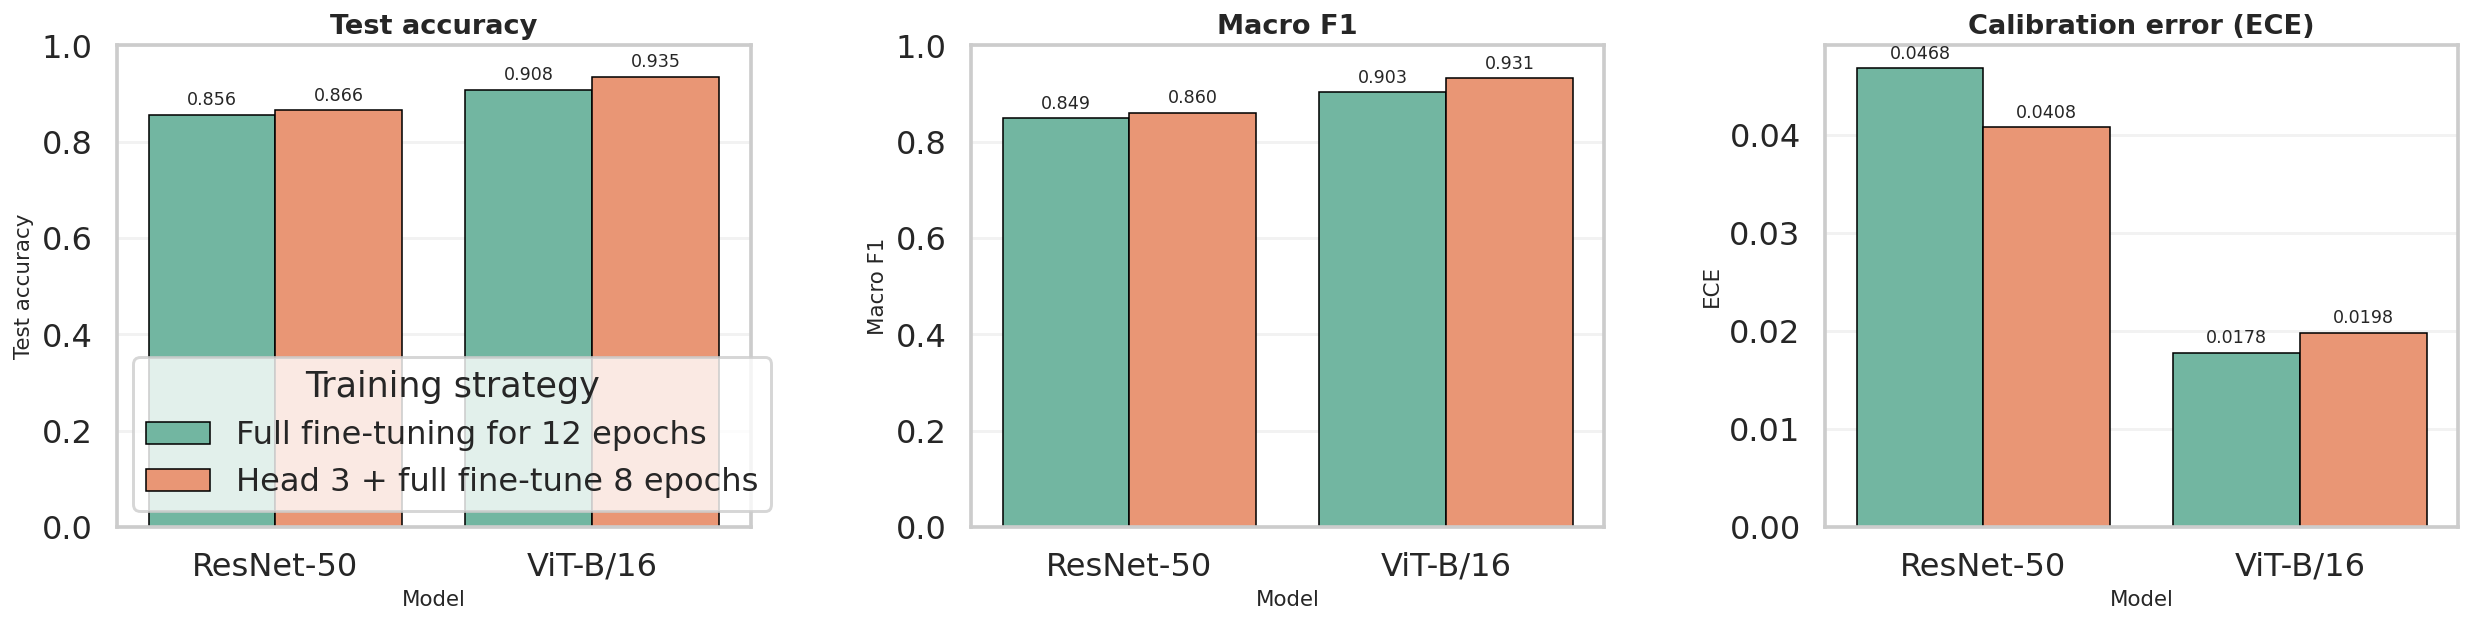
\includegraphics[width=0.86\textwidth]{stanforddogs_comparison_overview.png}
\caption{Overview figure exported from the fair four-run benchmark.}
\label{fig:stanforddogs_comparison_overview}
\end{figure}

\noindent \textbf{Discussion} Several observations follow from these results. First, \textbf{ViT-B/16} achieves the highest absolute accuracy and macro F1, with the staged strategy reaching 93.48\% accuracy and 0.9311 macro F1. Second, the \textbf{staged strategy} improves both families relative to full fine-tuning, suggesting that head warm-up before full unfreezing is beneficial on this fine-grained benchmark. Third, \textbf{ResNet-50} remains significantly lighter and faster to train than ViT-B/16, but its final accuracy is lower. This establishes a clear trade-off between efficiency and absolute performance.\\

\noindent \textbf{Calibration analysis} The staged runs are also the best-per-family models from the exported benchmark files, so their reliability diagrams are shown below.

\begin{figure}[H]
\centering
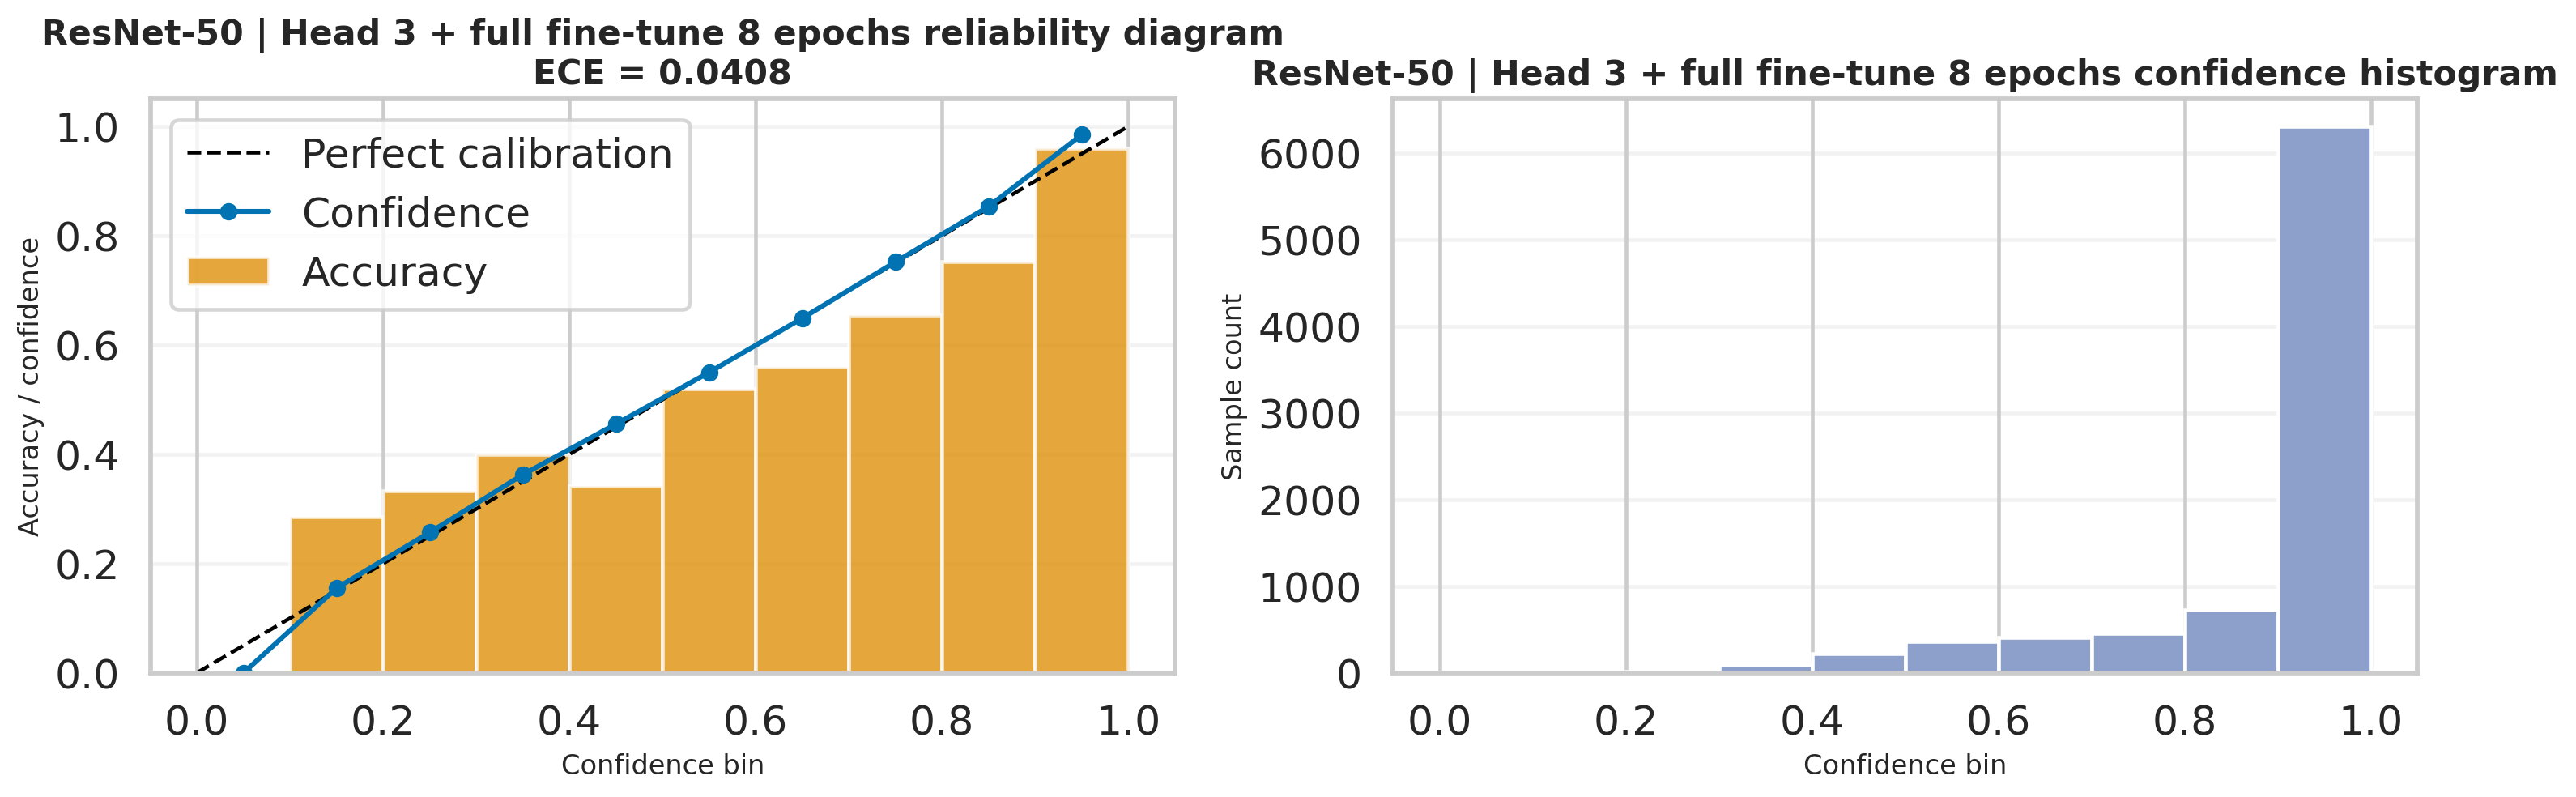
\includegraphics[width=0.9\textwidth]{resnet50_calibration_staged.png}
\caption{ResNet-50 staged calibration on Stanford Dogs (ECE = 0.0408).}
\label{fig:resnet50_calibration_staged}
\end{figure}

\begin{figure}[H]
\centering
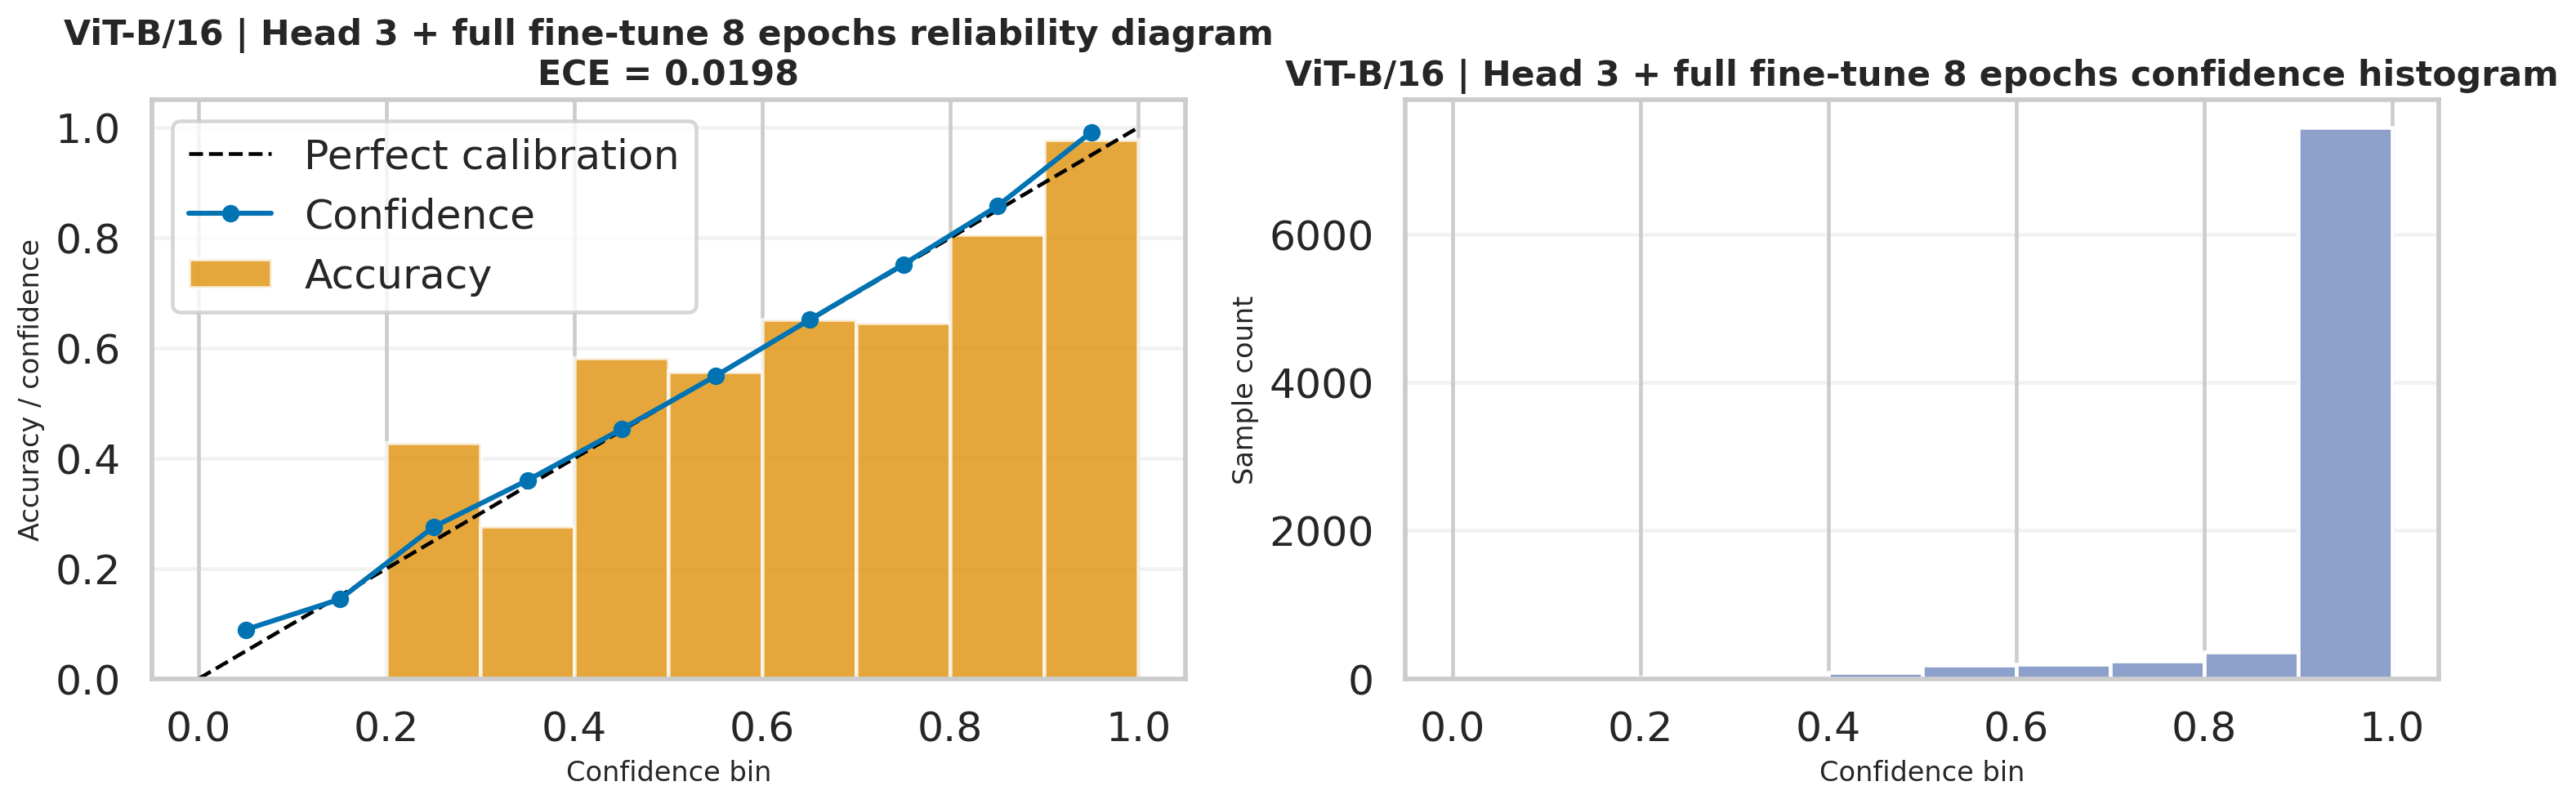
\includegraphics[width=0.9\textwidth]{vit_b16_calibration_staged.png}
\caption{ViT-B/16 staged calibration on Stanford Dogs (ECE = 0.0198).}
\label{fig:vitb16_calibration_staged}
\end{figure}

\noindent \textbf{Interpretation} ViT-B/16 is not only more accurate but also better calibrated than ResNet-50 in the final benchmark. Nevertheless, the CNN baseline remains useful because it is lighter, faster, and easier to deploy in constrained environments.

\subsubsection{Other Extension Reports}
\noindent \textbf{Interpretability} In addition to metrics, the notebook exports qualitative explanation artifacts for the best staged runs. For ResNet-50, Grad-CAM highlights the local regions that most influence breed prediction. For ViT-B/16, the attention gallery visualizes the spatial emphasis of the CLS-token attention pattern. These artifacts are useful for checking whether the models focus on semantically meaningful dog regions rather than background shortcuts.

\begin{figure}[H]
\centering
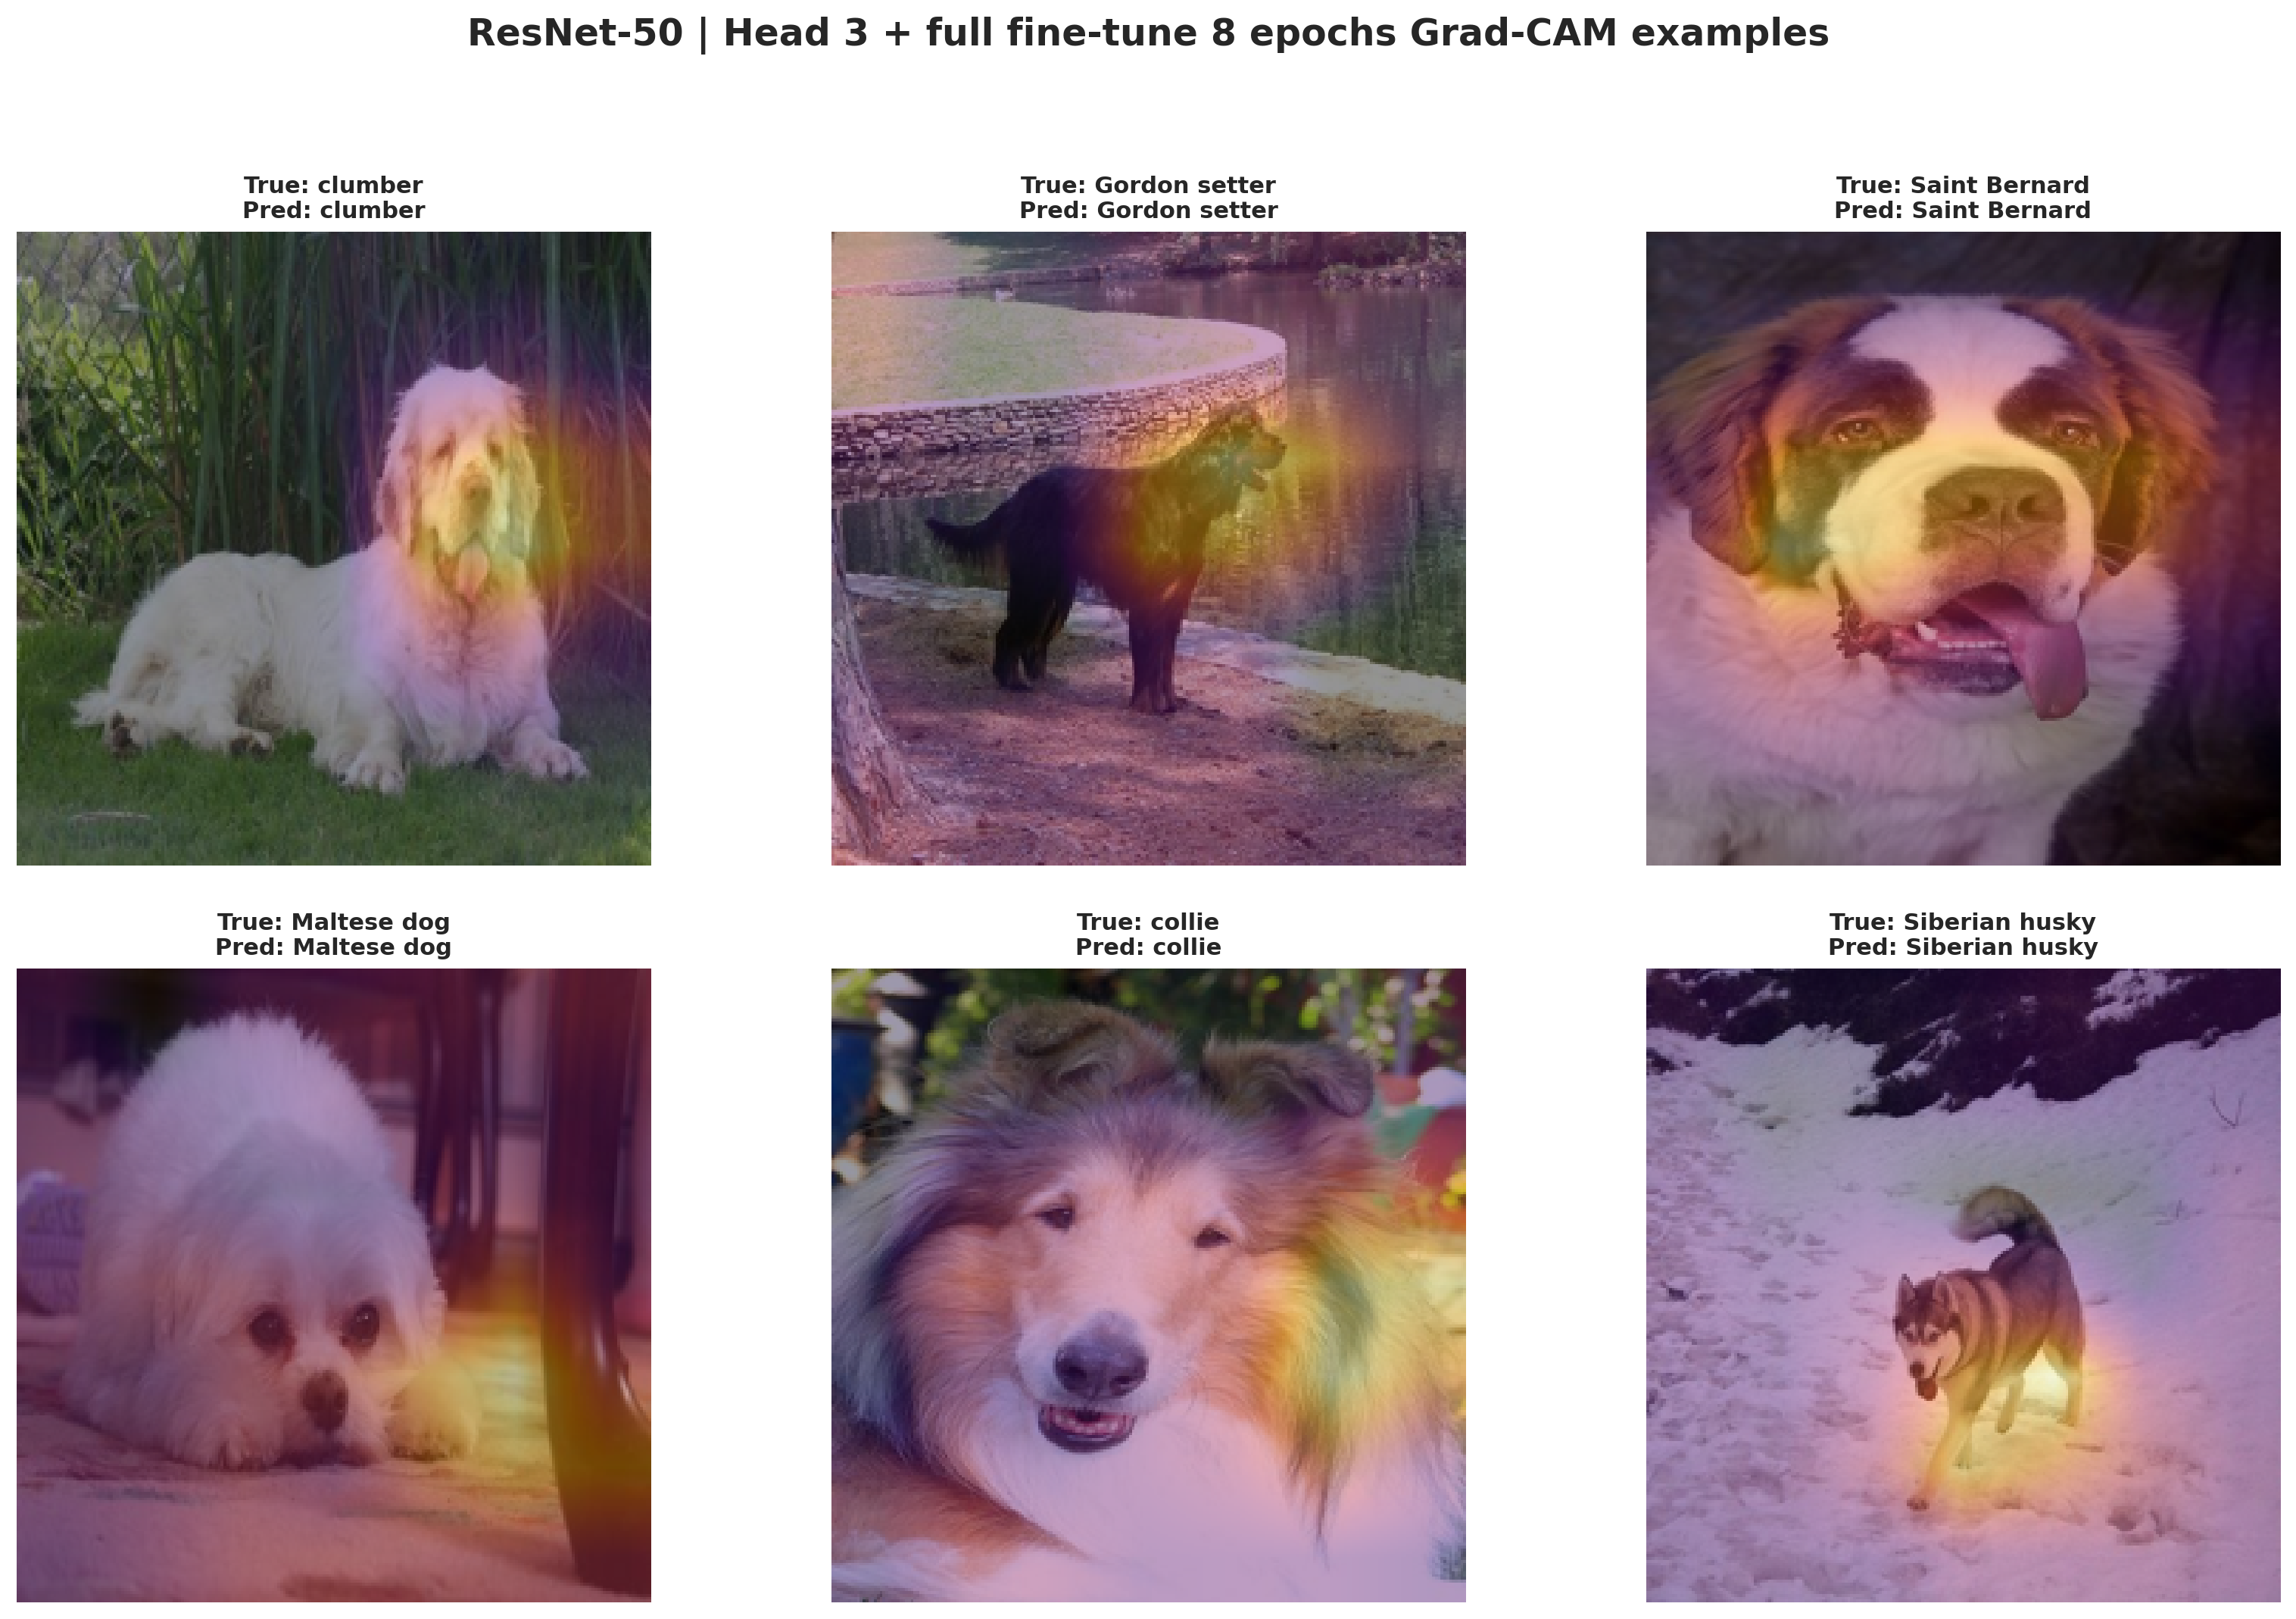
\includegraphics[width=0.92\textwidth]{resnet50_gradcam_gallery_staged.png}
\caption{Grad-CAM gallery for the staged ResNet-50 model on Stanford Dogs.}
\label{fig:resnet50_gradcam_gallery_staged}
\end{figure}

\begin{figure}[H]
\centering
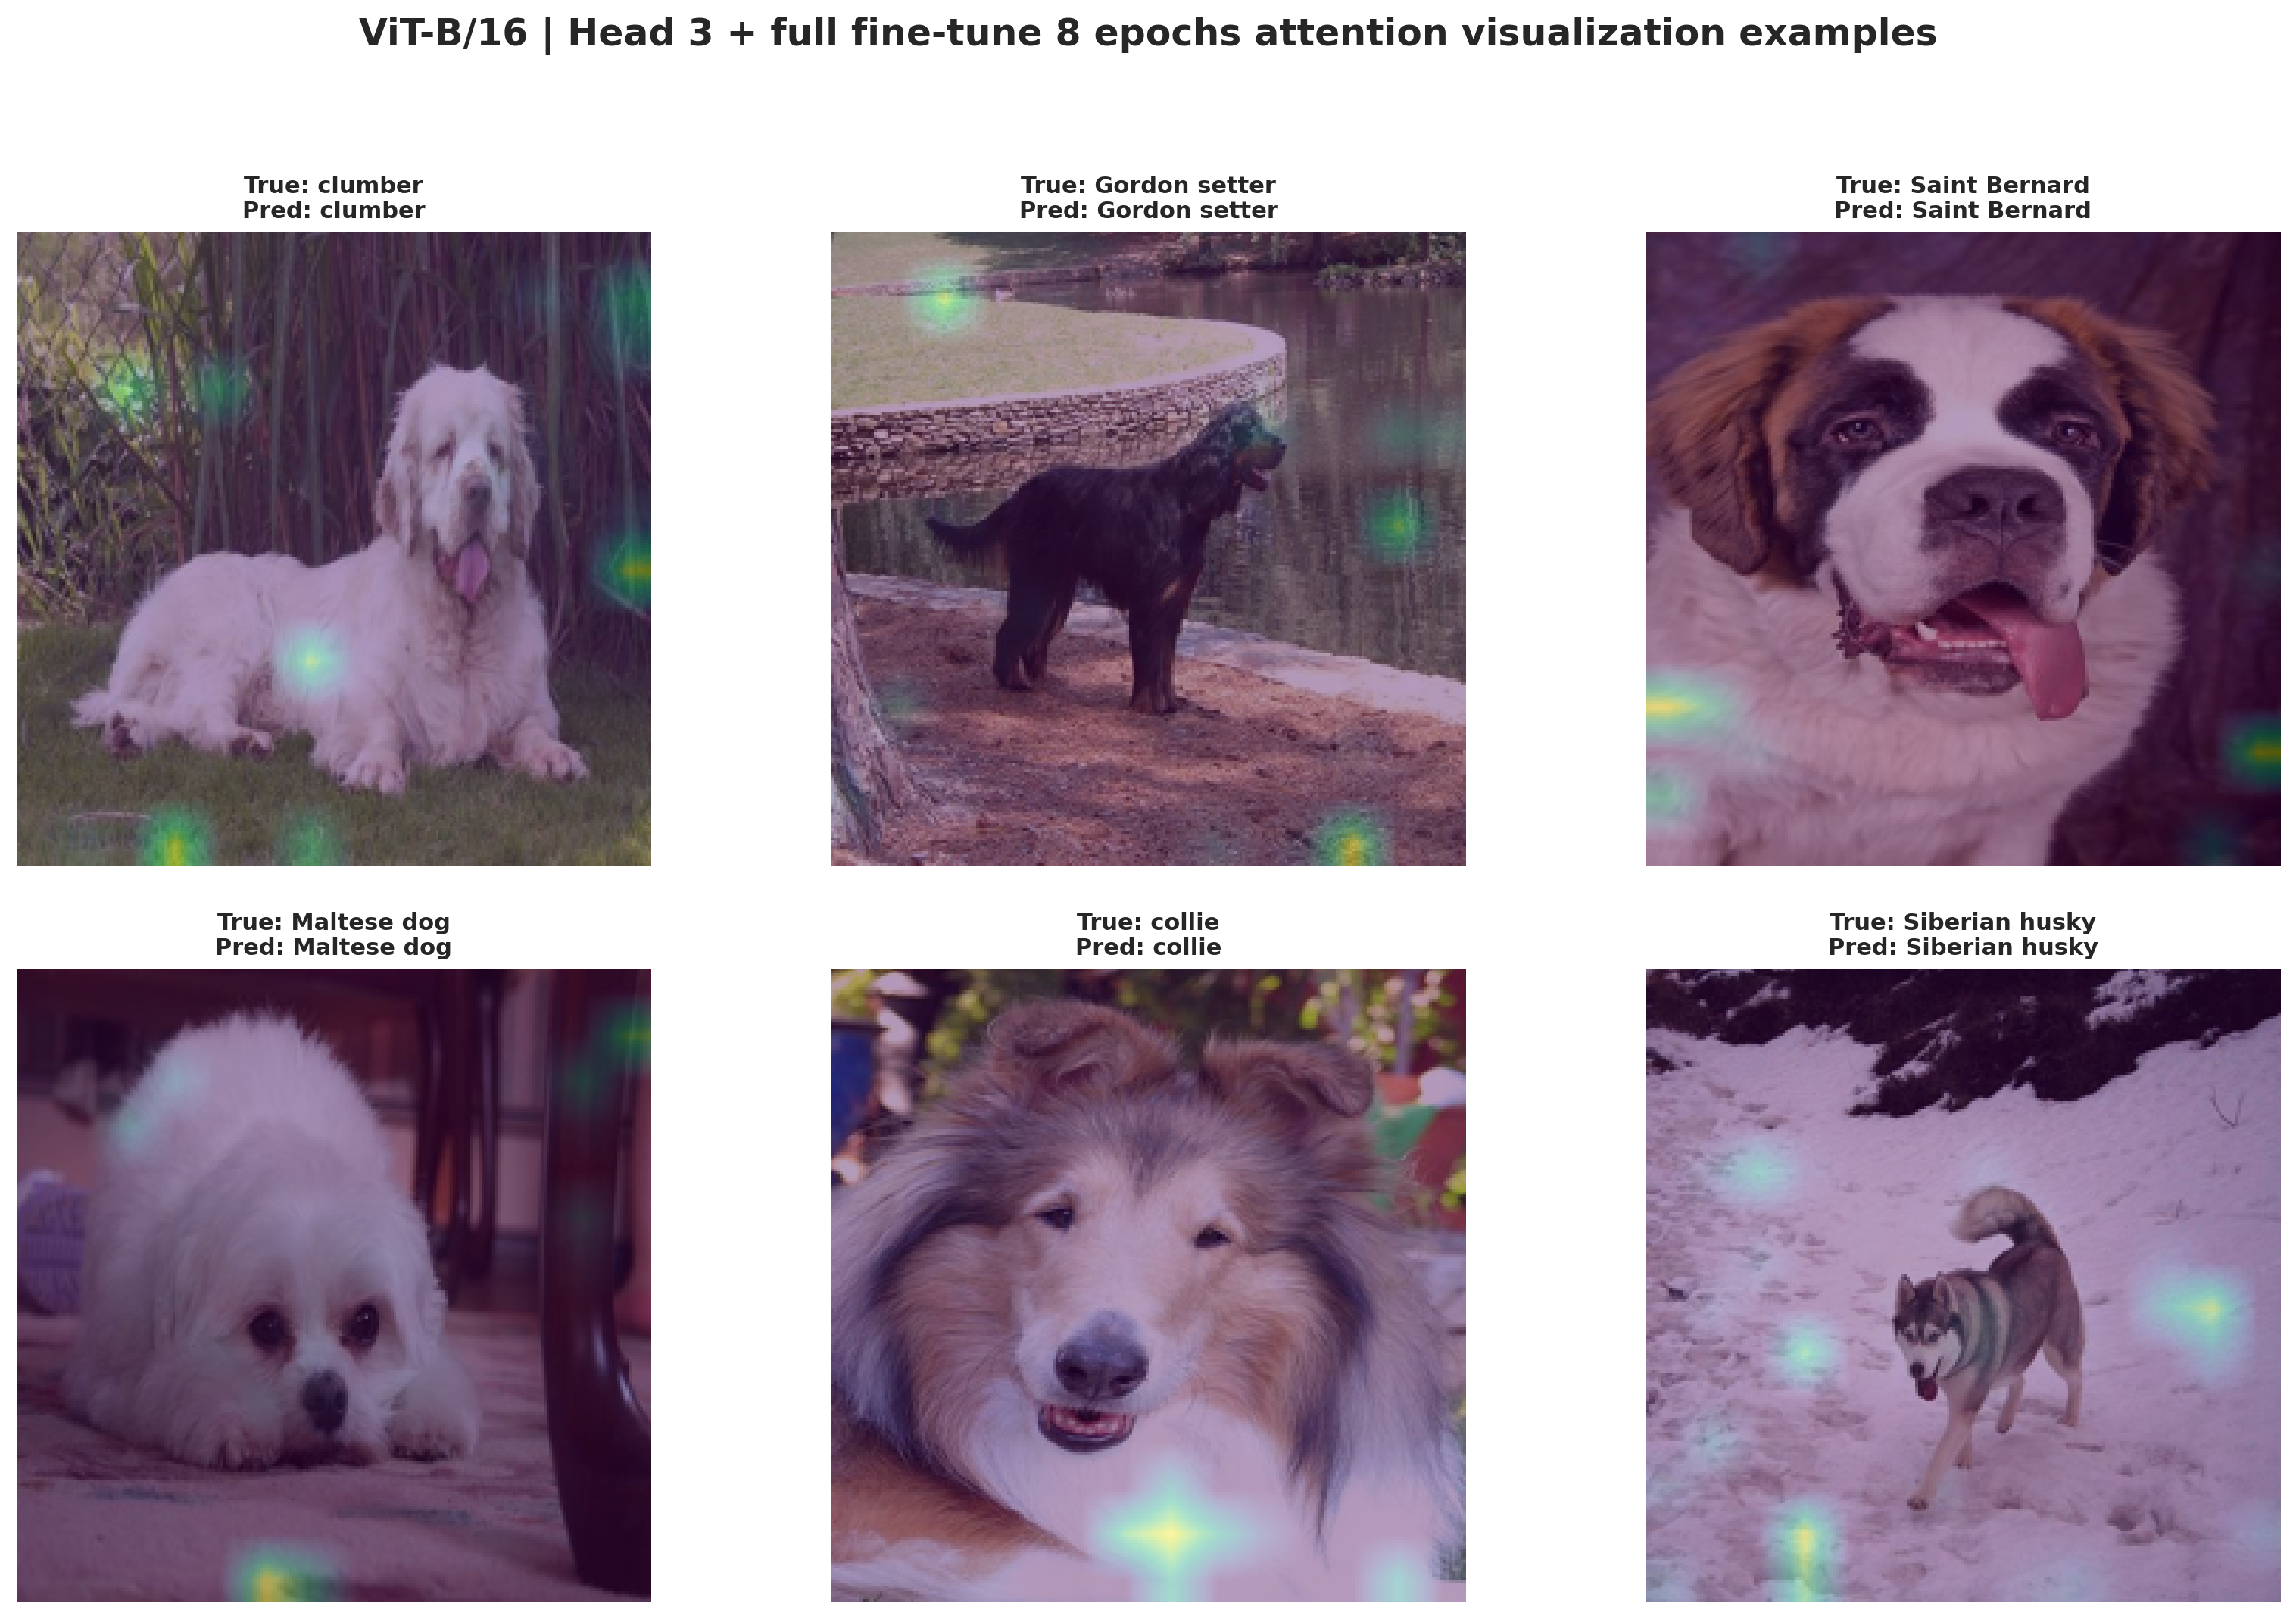
\includegraphics[width=0.92\textwidth]{vit_b16_attention_gallery_staged.png}
\caption{Attention gallery for the staged ViT-B/16 model on Stanford Dogs.}
\label{fig:vit_b16_attention_gallery_staged}
\end{figure}

\clearpage
\subsection{Text Track --- 20 Newsgroups, BiLSTM + Attention, and Transformer Fine-tuning}

\subsubsection{Problem Statement - Exploratory Data Analysis}
\noindent \textbf{Problem Statement} There are diversities of papers, newsletter, books... with various genres. We are not, however, able to manually distinguish between them in a short time. Therefore, RNN-based LSTM and Transformer-based DistilBERT are both taken into account to estimate the accuracy of classifying categories of each document based on natural language input.


\noindent \textbf{Dataset information} In this classification task, after examining a wide range of datasets, we determined to use the \texttt{20 Newsgroups} dataset as the primary dataset for the NLP-based topic classification task. With exactly 20 classes and over 18,000 documents, this dataset satisfies all the course requirements. The dataset details are as follows:

\begin{table}[H]
\centering
\caption{Corpus Statistics}
\begin{tabular}{lr}
\toprule
\textbf{Statistic} & \textbf{Value / Info} \\
\midrule
Total words & 3,423,145 \\
Total characters & 22,043,554 \\
Min docs/class & 628 (talk.religion.misc) \\
Max docs/class & 999 (rec.sport.hockey) \\
Mean docs/class & 942.3 \\
Std & 97.0 \\
\bottomrule
\end{tabular}
\end{table}

\begin{table}[H]
\centering
\caption{Per-document Word Count}
\begin{tabular}{lr}
\toprule
\textbf{Metric} & \textbf{Value} \\
\midrule
Mean & 181.6 \\
Median & 83.0 \\
Std & 501.3 \\
Min & 0 \\
Max & 11765 \\
\bottomrule
\end{tabular}
\end{table}


\begin{figure}[H]
\centering
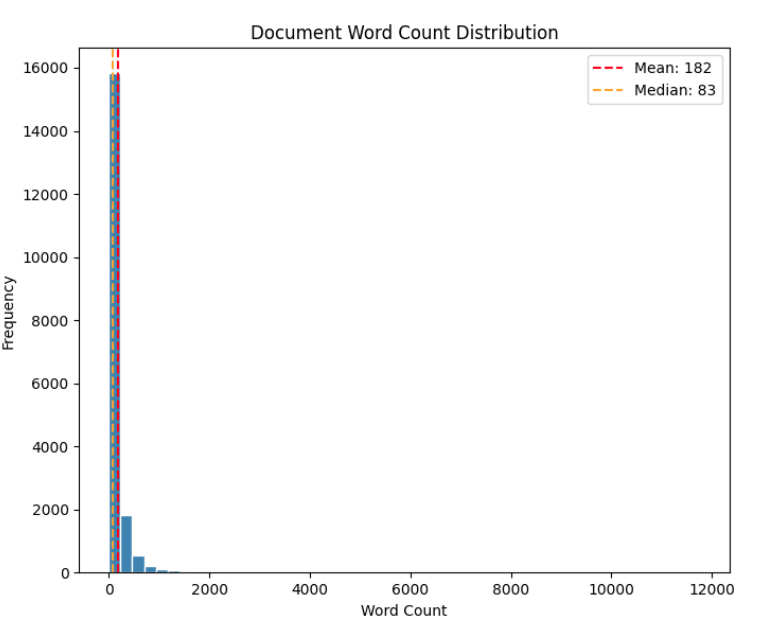
\includegraphics[width=0.8\textwidth]{wc_freq.png}
\caption{Word-frequency visualization from the EDA section.}
\label{fig:wc_freq}
\end{figure}

\begin{figure}[H]
\centering
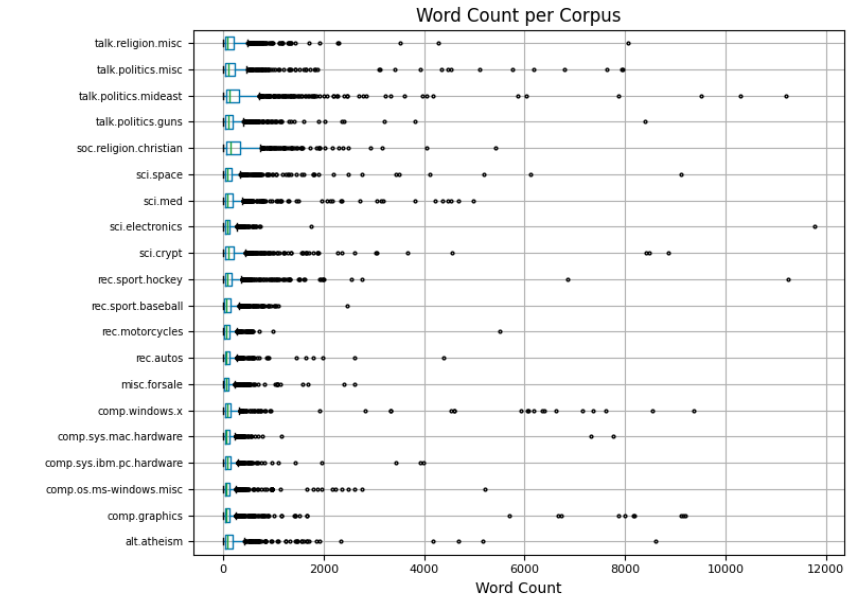
\includegraphics[width=0.85\textwidth]{wc_cor.png}
\caption{Word-correlation / corpus visualization from the EDA section.}
\label{fig:wc_cor}
\end{figure}

\subsubsection{Dataset, DataLoader, and Setup}
\noindent \textbf{Dataset overview} To ensure reliable access to the dataset, we downloaded it from Hugging Face. We then split 60\% of the data into a training set and used the remaining 40\% as the test set. Finally, we observe a moderate class imbalance, with the number of documents per class ranging from 628 to 999. \\ 

\noindent \textbf{Cleaning and Truncation} To obtain clean data prior to training, we applied several preprocessing strategies. After extensive experimentation, we found that the most effective pipeline removes quoted text, email headers, and signatures. In addition, we discard short documents containing fewer than 50 characters and truncate each document to a maximum of 400 words to better fit the BERT input constraint (512 tokens). \\ 

\noindent \textbf{Splitting strategy} The fine-grained data splitting strategy is shown below.

\begin{table}[H]
\centering
\caption{Train/Validation/Test Split}
\begin{tabular}{lrl}
\toprule
\textbf{Split} & \textbf{Samples} & \textbf{Note} \\
\midrule
Train & 8,584 & Stratified \\
Validation & 2,146 & Stratified \\
Test & 7,112 & Stratified \\
\bottomrule
\end{tabular}
\end{table}

\noindent \textbf{Tokenizer details} We adopt the \texttt{distilbert-base-uncased} tokenizer in our pipeline. Dynamic padding is applied via \texttt{DataCollatorWithPadding} to avoid unnecessary memory consumption. Approximately 90\% of the documents fit within the 512-token limit. \\ 

\noindent \textbf{Weighted loss} Due to class imbalance, we apply a weighting scheme to mitigate model bias. The loss function is defined as follows:

\begin{equation}
w_c = \frac{N}{C \cdot n_c}
\end{equation}
\begin{equation}
\mathcal{L} = \text{CrossEntropy}(x, y; w_c)
\end{equation}

\noindent where $N$ is the total number of samples, $C$ is the number of classes, and $n_c$ is the number of samples in class $c$. The weight $w_c$ is inversely proportional to the class frequency, giving higher importance to underrepresented classes. \\

\noindent \textbf{Batch setup} Due to the high computational cost of training BERT, we use a batch size of 12 for the training set and 36 for both the validation and test sets. As described earlier, token sequences are dynamically padded to match the maximum sequence length within each batch. \\ 

\subsubsection{Model Building, Training, Evaluation, and Comparison}
\noindent \textbf{BiLSTM with Attention} 

\noindent \textit{Architecture} We employ a Bidirectional Long Short-Term Memory (BiLSTM) model with an attention mechanism for text classification. The input tokens are first mapped to 300-dimensional GloVe embeddings, achieving approximately 43.3\% vocabulary coverage. These embeddings are further weighted using TF-IDF to emphasize informative terms.

\noindent The backbone consists of a two-layer BiLSTM encoder, which captures both forward and backward contextual dependencies in the sequence. On top of the encoder, an attention layer is applied to aggregate token-level representations into a context-aware document representation, allowing the model to focus on the most relevant parts of the input text. The resulting representation is then fed into a fully connected layer for classification. \\ 


\noindent \textbf{DistilBERT}

\noindent \textit{Model building} We utilize the pretrained \texttt{distilbert-base-uncased} model as the backbone for our classification task. DistilBERT is a lightweight transformer-based model that retains most of BERT's performance while being more computationally efficient.

\noindent The model is fine-tuned on our dataset by adding a classification head on top of the [CLS] token representation. During training, the entire model is updated end-to-end. This approach enables the model to leverage rich contextual representations learned during pretraining while adapting to the specific downstream classification task.


\subsubsection{Experimental Results, Figures, Analysis, and Discussion}
\noindent \textbf{DistilBERT Performance} After training, the model was evaluated on the held-out test set (7,112 samples) using multiple metrics to provide a comprehensive view of classification performance.
\begin{table}[H]
\centering
\small
\begin{tabular}{lc}
\toprule
\textbf{Metric} & \textbf{Value} \\
\midrule
Accuracy     & 73.88\% \\
F1 Macro     & 0.7268 \\
F1 Weighted  & 0.7400 \\
Precision    & 0.7299 \\
Recall       & 0.7258 \\
Best class   & rec.sport.hockey (F1: 0.93) \\
Worst class  & talk.religion.misc (F1: 0.32) \\
\bottomrule
\end{tabular}
\caption{Test results on the evaluation set.}
\label{tab:test_results_bert}
\end{table}


\begin{figure}[H]
\centering

\includegraphics[width=0.75\textwidth]{distilBERT_cfm.png}
\caption{DistilBERT confusion matrix.}
\label{fig:distilbert_confusion_matrix}
\end{figure}


\newpage
\noindent \textbf{BiLSTM with Attention} The BiLSTM model was evaluated after 20 epochs, reaching its peak validation accuracy of 69.72\% at epoch 18.

\begin{table}[H]
\centering
\small
\begin{tabular}{lc}
\toprule
\textbf{Metric} & \textbf{Score} \\
\midrule
Accuracy      & 62.90\% \\
F1 Macro      & 0.6179 \\
F1 Weighted   & 0.6311 \\
Precision     & 0.6251 \\
Recall        & 0.6155 \\
Best Class    & rec.sport.hockey (F1: 0.89) \\
Worst Class   & talk.religion.misc (F1: 0.19) \\
\bottomrule
\end{tabular}
\caption{Test results on the evaluation set.}
\label{tab:bilstm_results_lstm}
\end{table}

\begin{figure}[H]
\centering
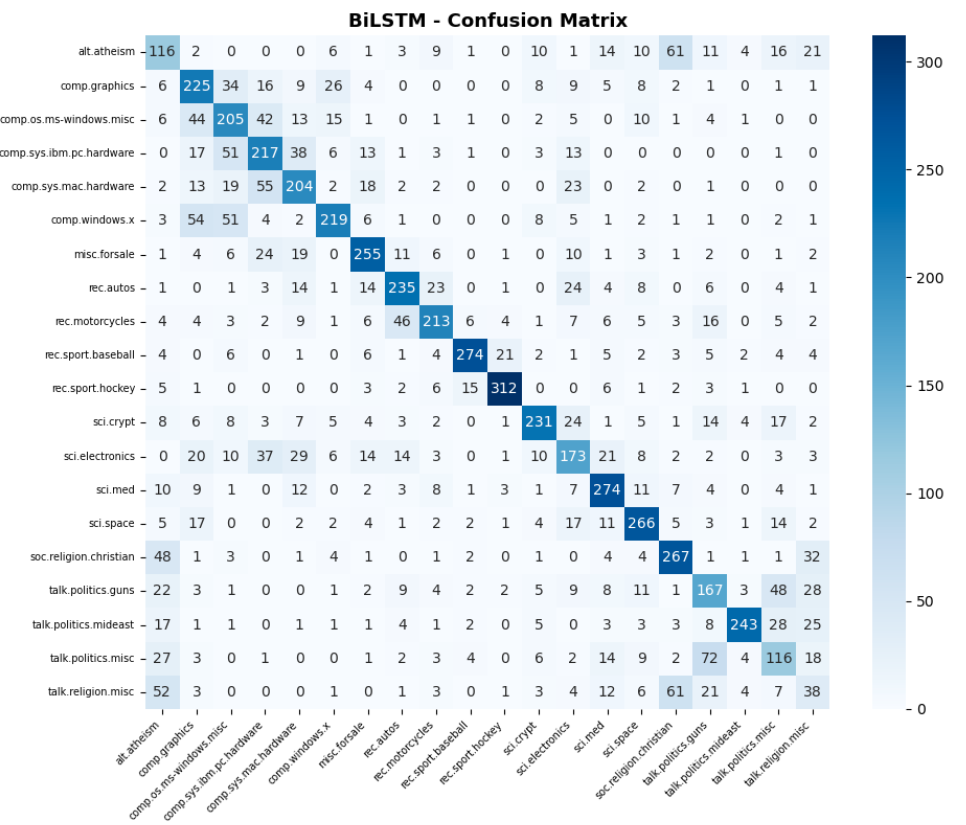
\includegraphics[width=0.75\textwidth]{lstm_cfm.png}
\caption{BiLSTM + Attention confusion matrix.}
\label{fig:bilstm_attention_confusion_matrix}
\end{figure}

\noindent \textbf{Key Insights} Our experiments reveal several important insights. First, a small but consistent gap between validation and test accuracy (e.g., 78.89\% vs.\ 73.88\%) indicates mild overfitting, likely due to the limited training size and class diversity. Second, class imbalance remains a key challenge: while class weighting improves recall for underrepresented categories, classes such as \textit{talk.religion.misc} and \textit{talk.politics.misc} still exhibit low performance. Third, model performance is strongly influenced by semantic separability: categories with clear topical boundaries (e.g., \textit{rec.sport.hockey}, \textit{sci.space}) achieve high F1 scores, whereas semantically overlapping classes lead to frequent confusion. Finally, error analysis shows systematic misclassification patterns driven by lexical overlap (e.g., religion-related classes), topic ambiguity in political discussions, and lack of distinctive keywords in short technical texts, highlighting limitations in contextual understanding across both RNN- and Transformer-based models.\\


\noindent \textbf{Systematic Comparison}
We compare DistilBERT (67M parameters) with an LSTM-based model to evaluate the impact of transformer architectures and self-attention mechanisms on text classification performance.
For transformer models, we evaluate three fine-tuning strategies: (i) freezing the backbone and training only the classification head, (ii) full fine-tuning, and (iii) a hybrid approach that progressively unfreezes layers. We assess model efficiency using accuracy, F1 score, training time, inference latency, and parameter count to quantify the trade-off between performance and computational cost.\\

\begin{table}[t]
\centering
\small
\begin{tabular}{lcccccc}
\toprule
Model & Val Acc & Test Acc & F1 Macro & Train (s) & Inf (ms) & Params \\
\midrule
DistilBERT (Hybrid) & 78.89 & 73.88 & 72.68 & 735 & 44.1 & 67M \\
BiLSTM + Attention & 69.72 & 62.90 & 0.6179 & 85 & -- & 15.8M \\
\bottomrule
\end{tabular}
\caption{Comparison between transformer and RNN-based models.}
\label{tab:comparison}
\end{table}

\noindent \textbf{Key Findings: Transformer vs RNN}
The results highlight a clear performance gap of approximately 11\% accuracy between BiLSTM and DistilBERT. This demonstrates the importance of contextualized representations, which static embeddings (e.g., GloVe) fail to capture. While attention improves the BiLSTM baseline, it does not fully compensate for the lack of bidirectional contextual pretraining. However, BiLSTM remains significantly more efficient, training up to 8--10$\times$ faster, making it a viable option in resource-constrained settings.

\subsubsection{Other Extension Reports}
\noindent \textbf{Fine-tuning Strategy Comparison} We compare three fine-tuning strategies (freeze backbone, hybrid, and full fine-tuning) on DistilBERT and BERT-base. Results show that full fine-tuning generally achieves the best performance, while the hybrid approach remains competitive and in some cases yields the highest test accuracy (e.g., BERT-base). In contrast, freezing the backbone significantly degrades performance, highlighting the importance of adapting pretrained representations. DistilBERT offers a strong efficiency--performance trade-off with fewer parameters and lower training cost, whereas BERT-base attains slightly higher peak accuracy.
\begin{table*}[t]
\centering
\small
\begin{tabular}{llcccccc}
\toprule
Model & Strategy & Val Acc & Test Acc & F1 Macro & Train (s) & Inf (ms) & Params \\
\midrule
DistilBERT & Freeze backbone & 67.38 & 66.15 & -- & 292  & 44.3 & 66.9M \\
DistilBERT & Hybrid          & 78.89 & 73.88 & 72.68 & 735  & 44.1 & 66.9M \\
DistilBERT & Full fine-tune  & \textbf{79.33} & 74.06 & \textbf{0.7406} & 644  & 44.4 & 66.9M \\
\midrule
BERT-base  & Freeze backbone & 64.80 & 62.93 & -- & 501  & 88.2 & 109.5M \\
BERT-base  & Hybrid          & 79.86 & \textbf{74.77} & -- & 1337 & 88.3 & 109.5M \\
BERT-base  & Full fine-tune  & 79.96 & 74.17 & -- & 1168 & 87.9 & 109.5M \\
\bottomrule
\end{tabular}
\caption{Comparison of fine-tuning strategies on DistilBERT and BERT-base.}
\label{tab:finetune}
\end{table*}


\begin{figure}[H]
\centering
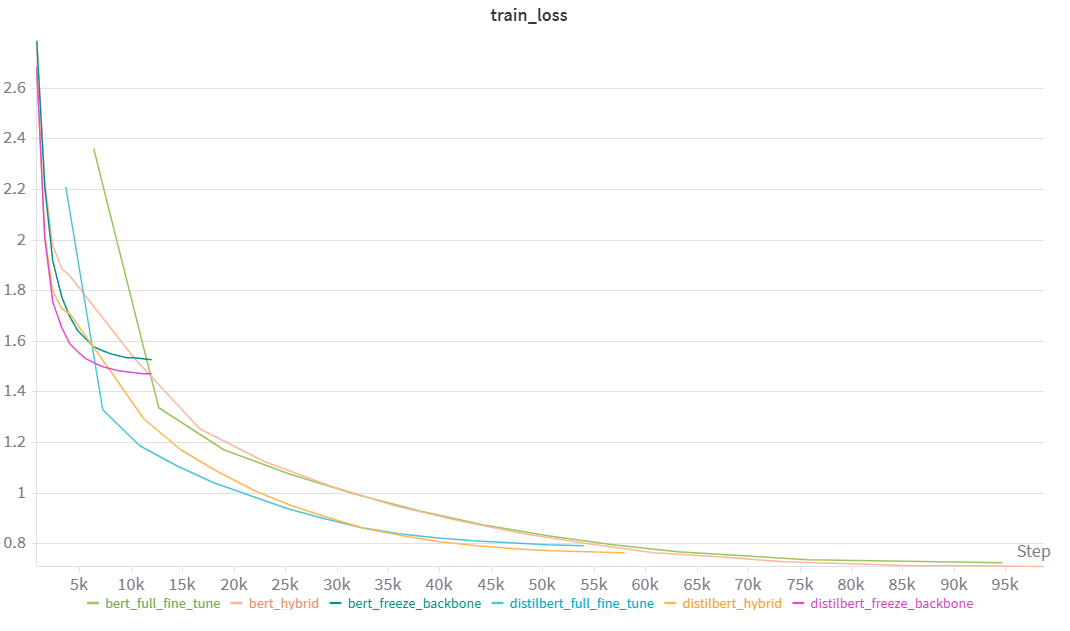
\includegraphics[width=0.7\textwidth]{loss.png}
\caption{Training-loss comparison for Transformer fine-tuning strategies.}
\label{fig:transformer_training_loss_comparison}
\end{figure}

\begin{figure}[H]
\centering
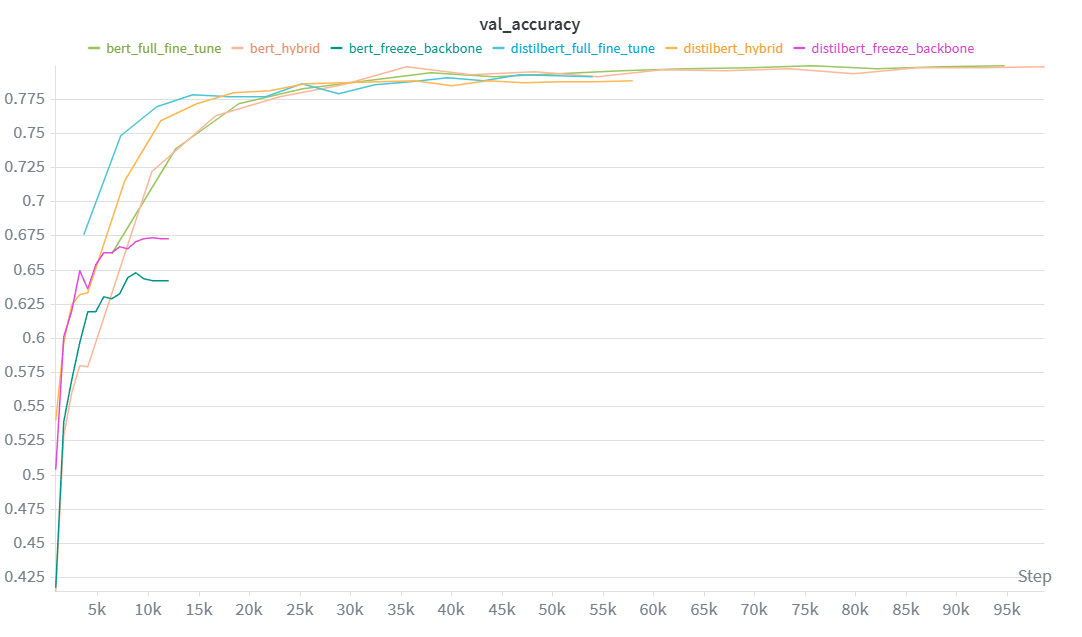
\includegraphics[width=0.7\textwidth]{val_acc.png}
\caption{Validation-accuracy comparison for Transformer fine-tuning strategies.}
\label{fig:transformer_validation_accuracy_comparison}
\end{figure}


\noindent \textbf{Model Efficiency Comparison}
We evaluate model efficiency by comparing DistilBERT and BERT-base across key metrics including parameter count, test accuracy, training time, and inference latency. The goal is to analyze the trade-off between computational cost and performance under knowledge distillation. DistilBERT is obtained by compressing BERT-base through a distillation process during pretraining, reducing model depth and size while preserving most of the predictive capability. We report both absolute values and relative ratios to highlight efficiency gains.

\begin{table}[H]
\centering
\small
\begin{tabular}{lccc}
\toprule
\textbf{Metric} & \textbf{DistilBERT} & \textbf{BERT-base} & \textbf{Ratio} \\
\midrule
Parameters        & 66.9M   & 109.5M & 1.63$\times$ \\
Test Accuracy     & 73.88\% & 74.77\% & +0.89\% \\
F1 Macro          & 72.68   & --      & -- \\
Training Time     & 735s    & 1337s   & 1.82$\times$ \\
Inference Time    & 44.1ms  & 88.3ms  & 2.0$\times$ \\
\midrule
Encoder Layers    & 6       & 12      & 50\% \\
Parameter Reduction & 66.9M & 109.5M  & -39\% \\
Inference Speedup & 44.1ms  & 88.3ms  & 2.0$\times$ faster \\
Accuracy Drop     & 73.88\% & 74.77\% & -0.89\% \\
\bottomrule
\end{tabular}
\caption{Efficiency comparison between DistilBERT and BERT-base. DistilBERT retains most of BERT-base performance while reducing parameters and latency significantly.}
\label{tab:efficiency}
\end{table}


\clearpage
\subsection{Multimodal Results and Analysis}

\begin{figure}[H]
\centering
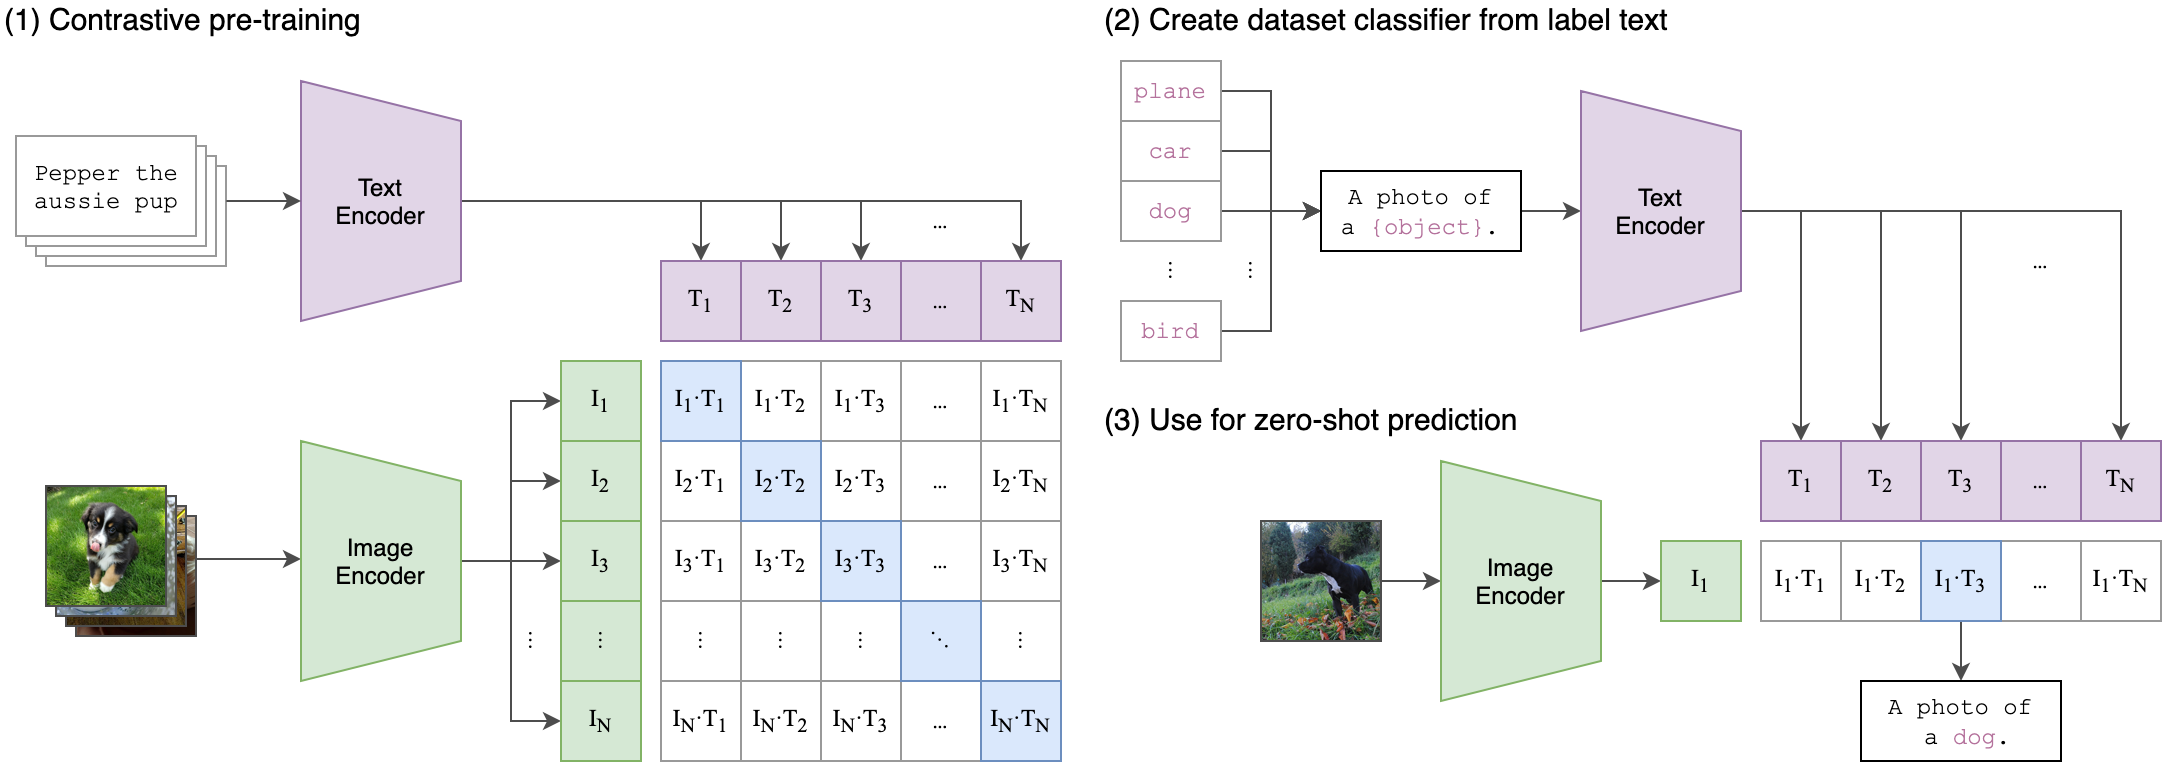
\includegraphics[width=0.72\textwidth]{CLIP.png}
\caption{CLIP backbone used for multimodal image-text learning.}
\label{fig:clip_backbone}
\end{figure}

\begin{center}
\small
\begin{tabular}{|l|l|c|c|}
\hline
\textbf{Backbone} & \textbf{Setting} & \textbf{Accuracy} & \textbf{F1} \\
\hline
ViT-B/16 & Zero-shot & 0.8959 & 0.8769 \\
\hline
ViT-B/16 & Best: Prototype + 10-shot + aug & 0.9224 & 0.9231 \\
\hline
RN50 & Zero-shot & 0.8680 & 0.8438 \\
\hline
RN50 & Best: Prototype + 5-shot + no\_aug & 0.8806 & 0.8825 \\
\hline
\end{tabular}
\end{center}

The multimodal experiments show that ViT-B/16 is more stable than RN50 across adaptation settings. Few-shot adaptation improves over zero-shot when support quality is sufficient. The \textbf{Prototype head} is generally more robust than the Linear head in low-shot conditions.

\begin{figure}[H]
\centering
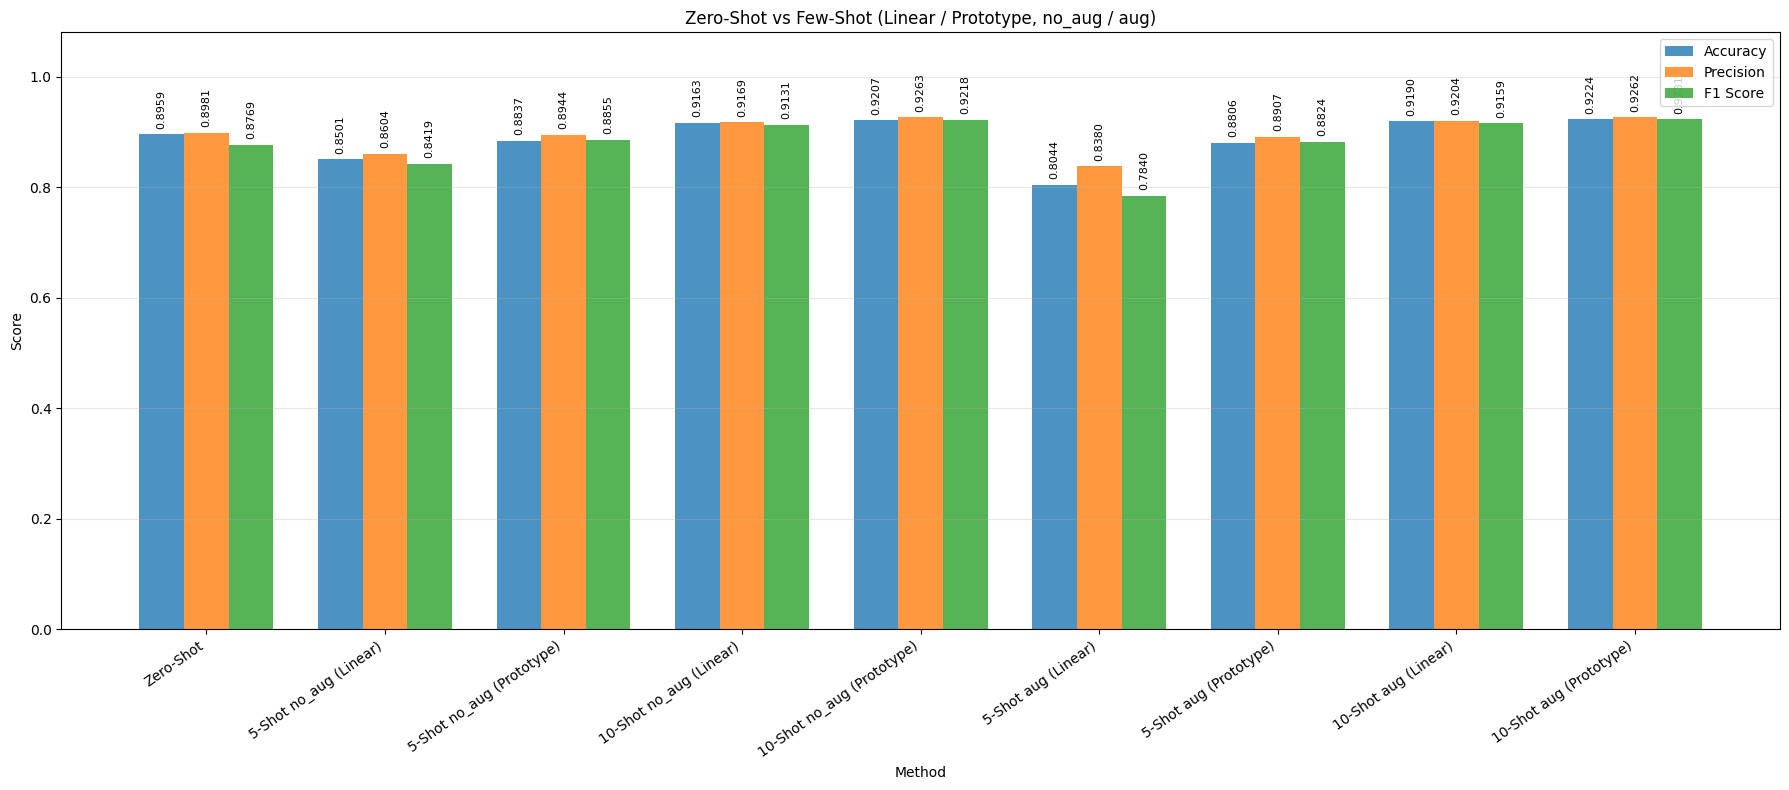
\includegraphics[width=0.75\textwidth]{accuracy.png}
\caption{ViT-B/16 zero-shot vs few-shot comparison.}
\label{fig:vitb16_zero_shot_few_shot}
\end{figure}

\begin{figure}[H]
\centering
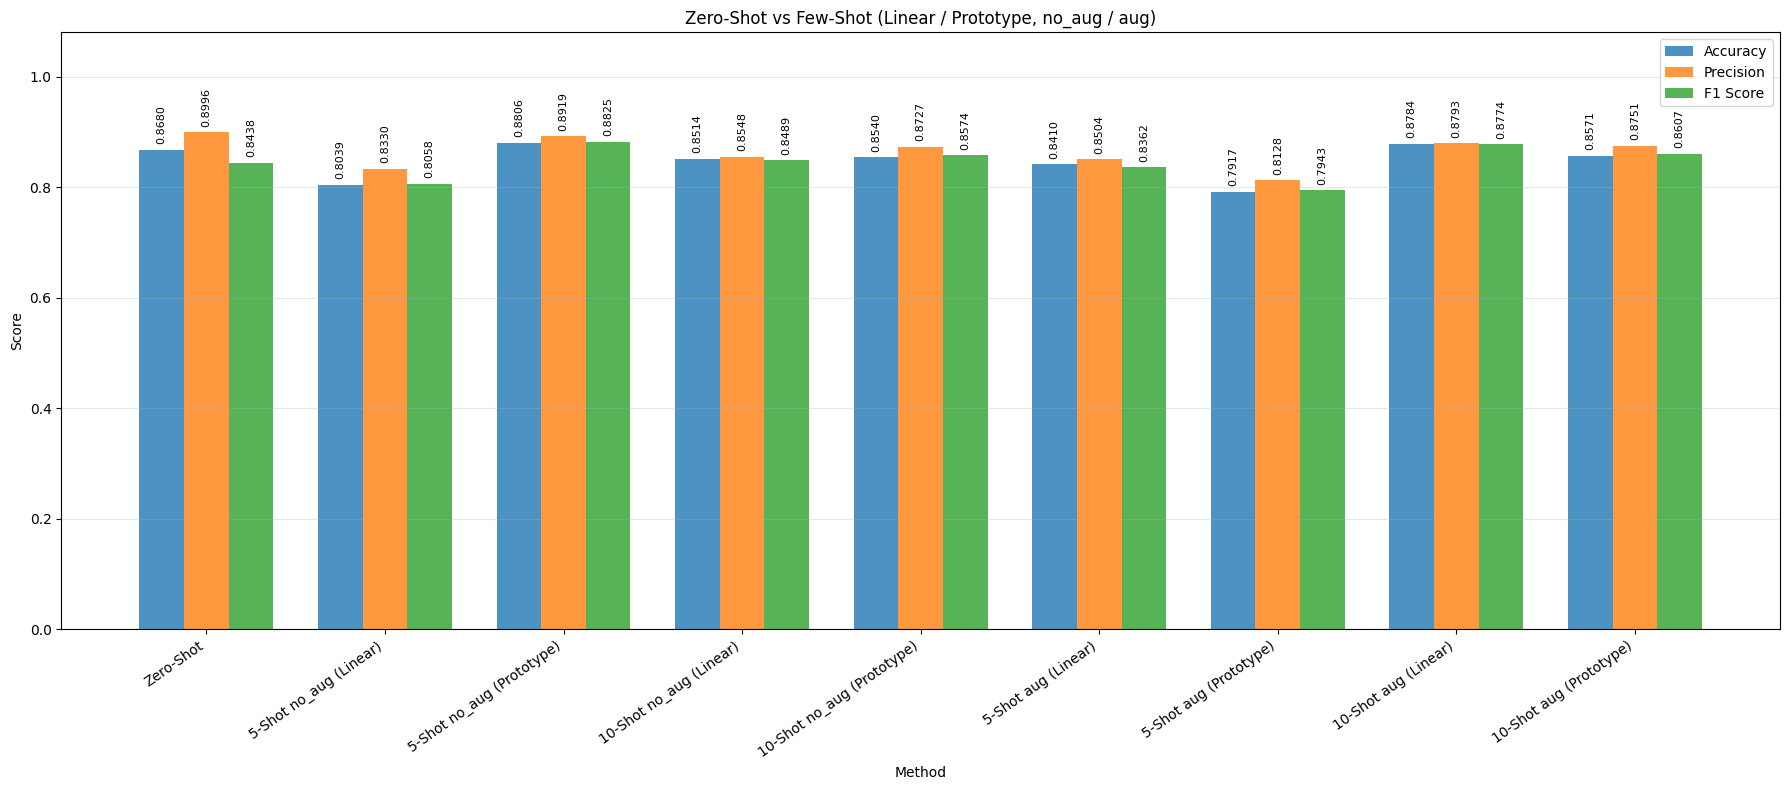
\includegraphics[width=0.75\textwidth]{method.png}
\caption{RN50 zero-shot vs few-shot comparison.}
\label{fig:rn50_zero_shot_few_shot}
\end{figure}

\begin{figure}[H]
\centering
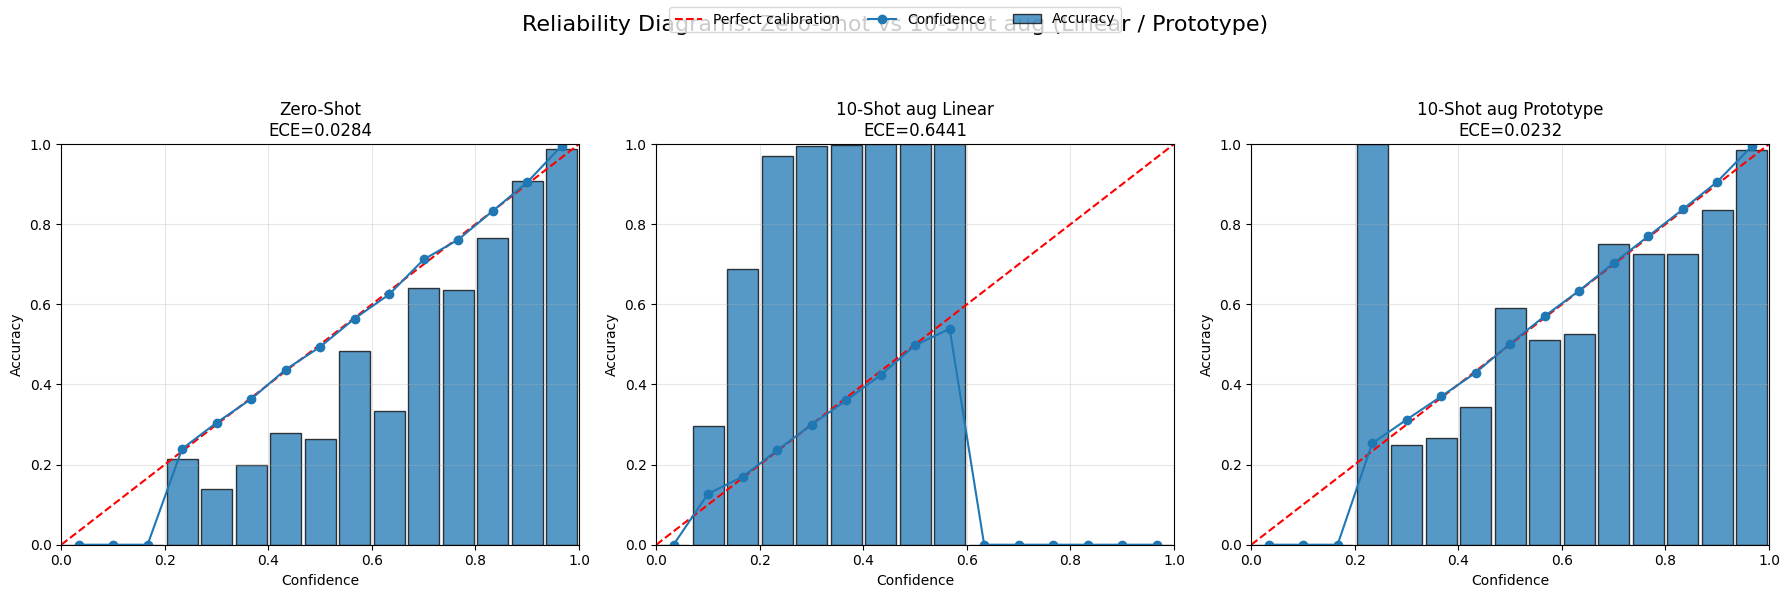
\includegraphics[width=0.75\textwidth]{ECE-vit16.png}
\caption{Calibration summary for ViT-B/16 settings.}
\label{fig:vitb16_calibration_summary}
\end{figure}

\begin{figure}[H]
\centering
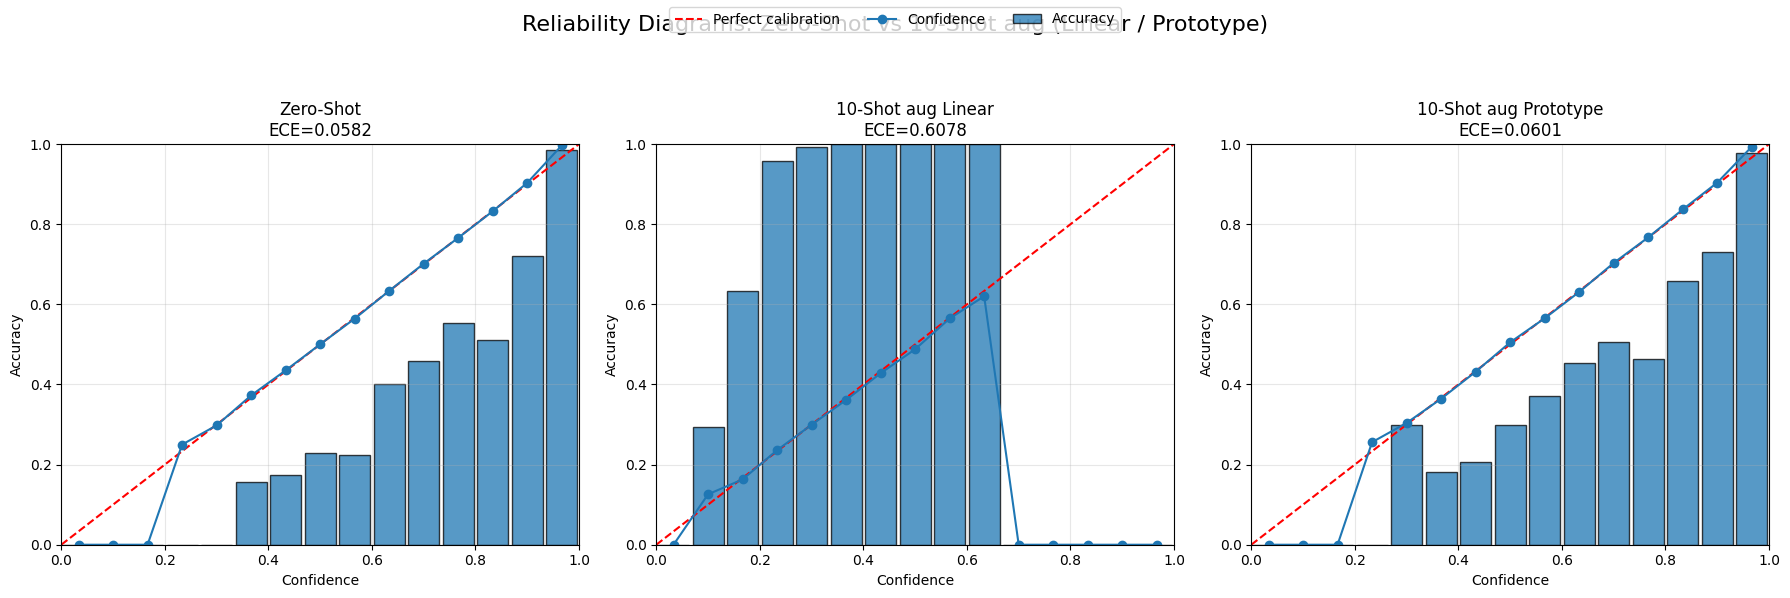
\includegraphics[width=0.75\textwidth]{ECE_resnet50.png}
\caption{Calibration summary for RN50 settings.}
\label{fig:rn50_calibration_summary}
\end{figure}

\section{Extensions}
Beyond the mandatory comparisons, we include additional analyses:
\begin{itemize}[leftmargin=*, nosep]
    \item \textbf{Image:} interpretability and calibration analysis.
    \item \textbf{Text:} fine-tuning strategy comparison and efficiency analysis.
    \item \textbf{Multimodal:} augmentation vs no-augmentation, calibration, and confusion-matrix-based error analysis.
\end{itemize}

\section{Conclusion}
This final report demonstrates that pretrained deep learning models can be effectively adapted across image, text, and multimodal classification tasks.
\begin{itemize}[leftmargin=*, nosep]
    \item In image classification on \textbf{Stanford Dogs}, \textbf{ViT-B/16} with the staged strategy achieves the highest accuracy, while \textbf{ResNet-50} remains the lighter and faster CNN baseline.
    \item In text classification, Transformer fine-tuning (DistilBERT) outperforms the RNN baseline, especially on semantically complex classes.
    \item In multimodal classification, \textbf{ViT-B/16 + Prototype few-shot} is the best overall setting, and zero-shot remains a strong baseline.
\end{itemize}
Overall, the required comparisons are completed with consistent metrics and analysis, and extensions provide additional insight into robustness, confidence, and practical deployment trade-offs.

\section{Project Links}
\begin{itemize}[leftmargin=*, nosep]
    \item GitHub Pages: \href{https://tanh1c.github.io/HAT-Deep_Learning/}{tanh1c.github.io/HAT-Deep\_Learning/}
    \item Image demo (Streamlit): \href{https://hat-deeplearning-tjflfkryrwcwsas6py8ta5.streamlit.app/}{hat-deeplearning-tjflfkryrwcwsas6py8ta5.streamlit.app/}
\end{itemize}

\section{Use of AI Assistants}
In adherence to the Ho Chi Minh City University of Technology -- VNU-HCM Ethics Policy, we did not employ AI assistants to generate the initial draft of this paper. We used AI assistants (GPT-5.2) exclusively at the sentence level to improve clarity and correct grammar.

\end{document}
